\usepackage{fancyhdr}
%\usepackage{mu}
\usepackage{wasysym}
\usepackage{bitset}% Preambel mit Einstellungen importieren
% Document type and used packages
\documentclass[open=right, % Sorgt für Umbruch bei Chapter (any erzeugt keine Leerseiten) -> Kapitel darf nur auf der rechten Seite beginnen
  paper=A4,               % DIN-A4-Papier
  a4paper,                % DIN-A4-Papier
  12pt,                   % Schriftgöße
  headings=small,         % Kleine Überschriften
  headsepline=true,       % Trennlinie am Kopf der Seite
  footsepline=false,      % Keine Trennlinie am Fuß der Seite
  bibliography=totoc,     % Literaturverzeichnis in das Inhaltsverzeichnis aufnehmen
  twoside=off,            % Für doppelseitigen Druck auf on stellen, off für einseitig
  DIV=7,                  % Verhältnis der Ränder zum bedruckten Bereich
  chapterprefix=false,     % Kapitel x vor dem Kapitelnamen
  cleardoublepage=plain]{scrbook}

% Pakete einbinden, die benötigt werden
\usepackage{scrlayer-scrpage}
\usepackage[utf8]{inputenc}       % Dateien in UTF-8 benutzen
\usepackage{longtable}
\usepackage[T1]{fontenc}          % Zeichenkodierung
\usepackage{graphicx}             % Bilder einbinden
\usepackage[main=ngerman, english]{babel}       % Deutsch und Englisch unterstützen
\usepackage{xcolor}               % Color support
\usepackage{amsmath}              % Matheamtische Formeln
\usepackage{amsfonts}             % Mathematische Zeichensätze
\usepackage{amssymb}              % Mathematische Symbole
\usepackage{float}                % Fließende Objekte (Tabellen, Grafiken etc.)
\usepackage{booktabs}             % Korrekter Tabellensatz
\usepackage[printonlyused, withpage, footnote]{acronym}  % Abkürzungsverzeichnis [nur verwendete Abkürzugen]
\usepackage{makeidx}              % Sachregister
\usepackage{listings}             % Source Code listings
\usepackage{listingsutf8}         % Listings in UTF8
\usepackage[hang,font={sf,footnotesize},labelfont={footnotesize,bf}]{caption} % Beschriftungen
\usepackage[scaled]{helvet}       % Schrift Helvetia laden
\usepackage[absolute]{textpos}	  % Absolute Textpositionen (für Deckblatt)
\usepackage{calc}                 % Berechnung von Positionen
\usepackage{blindtext}            % Blindtexte
\usepackage[bottom=40mm,left=35mm,right=35mm,top=30mm]{geometry} % Ränder ändern
\usepackage{setspace}             % Abstände korrigieren
\usepackage{ifthen}               % Logische Bedingungen mit ifthenelse
\usepackage{scrhack}              % Get rid of tocbasic warnings
\usepackage[pagebackref=false,german]{hyperref}  % Hyperlinks
\usepackage[all]{hypcap}          % Korrekte Verlinkung von Floats
\usepackage[autostyle=true,german=quotes]{csquotes}   % Zitate
\usepackage[backend=biber,
  isbn=true,                     % ISBN nicht anzeigen, gleiches geht mit nahezu allen anderen Feldern
  sortlocale=de_DE,               % Sortierung der Einträge für Deutsch
  %sortlocale=en_US,              % Sortierung der Einträge für Englisch
  autocite=inline,                % regelt Aussehen für \autocite (inline=\parancite)
  hyperref=true,                  % Hyperlinks für Ziate
  style=ieee                     % Zitate als Zahlen [1]
  %style=alphabetic               % Zitate als Kürzel und Jahr [Ein05]
  %style=authoryear                % Zitate Author und Jahr [Einstein (1905)]
  %style=LNI
]{biblatex}                       % Literaturverwaltung mit BibLaTeX
\usepackage{rotating}             % Seiten drehen
\usepackage{harveyballs}          % Harveyballs
\usepackage{tcolorbox}
\usepackage[export]{adjustbox}
\usepackage{subcaption}
\usepackage{color}
\usepackage{colortbl}
\usepackage{wrapfig}
\usepackage{todonotes}
\usepackage{tabularx}
\newcolumntype{b}{>{\hsize=1.2\hsize}X}
\newcolumntype{m}{>{\hsize=.5\hsize}X}
\newcolumntype{s}{>{\hsize=.3\hsize}X}
\newcolumntype{d}{>{\hsize=1.5\hsize}X}
\newcolumntype{c}{>{\hsize=.6\hsize}X}
\newcolumntype{a}{>{\hsize=.2\hsize}X}
\usepackage{tikz}


\setlength{\bibitemsep}{1em}     % Abstand zwischen den Literaturangaben
\setlength{\bibhang}{2em}        % Einzug nach jeweils erster Zeile

% Trennung von URLs im Literaturverzeichnis (große Werte [> 10000] verhindern die Trennung)
\defcounter{biburlnumpenalty}{10} % Strafe für Trennung in URL nach Zahl
\defcounter{biburlucpenalty}{500}  % Strafe für Trennung in URL nach Großbuchstaben
\defcounter{biburllcpenalty}{500}  % Strafe für Trennung in URL nach Kleinbuchstaben

% Farben definieren
\definecolor{linkblue}{RGB}{0, 0, 100}
\definecolor{linkblack}{RGB}{0, 0, 0}
\definecolor{comment}{RGB}{63, 127, 95}
\definecolor{darkgreen}{RGB}{14, 144, 102}
\definecolor{darkblue}{RGB}{0,0,168}
\definecolor{darkred}{RGB}{128,0,0}
\definecolor{javadoccomment}{RGB}{0,0,240}
\definecolor{Gray}{RGB}{242,242,242}

% Einstellungen für das Hyperlink-Paket
\hypersetup{
  colorlinks=true,      % Farbige links verwenden
  %    allcolors=linkblue,
  linktoc=all,          % Links im Inhaltsverzeichnis
  linkcolor=linkblack,  % Querverweise
  citecolor=linkblack,  % Literaturangaben
  filecolor=linkblack,  % Dateilinks
  urlcolor=linkblack    % URLs
}

% Einstellungen für Quelltexte
\definecolor{backcolour}{rgb}{0.95,0.95,0.92}
\definecolor{codegray}{rgb}{0.5,0.5,0.5}

%\usepackage[T1]{fontenc}
%\usepackage[scaled=0.85]{beramono}
\usepackage{xcolor}
\usepackage{listings}

\newcommand\JSONnumbervaluestyle{\color{blue}}
\newcommand\JSONstringvaluestyle{\color{red}}

% switch used as state variable
\newif\ifcolonfoundonthisline

\makeatletter

\lstdefinestyle{json}
{
  showstringspaces    = false,
  keywords            = {false,true},
  alsoletter          = 0123456789.,
  morestring          = [s]{"}{"},
  stringstyle         = \ifcolonfoundonthisline\JSONstringvaluestyle\fi,
  MoreSelectCharTable =%
    \lst@DefSaveDef{`:}\colon@json{\processColon@json},
  basicstyle          = \ttfamily,
  keywordstyle        = \ttfamily\bfseries,
}

% flip the switch if a colon is found in Pmode
\newcommand\processColon@json{%
  \colon@json%
  \ifnum\lst@mode=\lst@Pmode%
    \global\colonfoundonthislinetrue%
  \fi
}

\lst@AddToHook{Output}{%
  \ifcolonfoundonthisline%
    \ifnum\lst@mode=\lst@Pmode%
      \def\lst@thestyle{\JSONnumbervaluestyle}%
    \fi
  \fi
  %override by keyword style if a keyword is detected!
  \lsthk@DetectKeywords% 
}

% reset the switch at the end of line
\lst@AddToHook{EOL}%
  {\global\colonfoundonthislinefalse}
\lstdefinelanguage{JavaScript}{
  keywords={typeof, new, true, false, catch, function, return, null, catch, switch, var, if, in, while, do, else, case, break},
  keywordstyle=\color{blue}\bfseries,
  ndkeywords={class, export, boolean, throw, implements, import, this},
  ndkeywordstyle=\color{darkgray}\bfseries,
  identifierstyle=\color{black},
  sensitive=false,
  comment=[l]{//},
  morecomment=[s]{/*}{*/},
  commentstyle=\color{purple}\ttfamily,
  stringstyle=\color{red}\ttfamily,
  morestring=[b]',
  morestring=[b]"
}

\newtcolorbox{zitat}[1][]{%
  colback=block-gray,
  grow to right by=-1mm,
  boxrule=0pt,
  boxsep=0pt,
  breakable,
  enhanced jigsaw,
  borderline west={2pt}{0pt}{gray},
  colbacktitle={block-gray},
  coltitle={black},
  fonttitle={\large\bfseries},
  attach title to upper={},
  #1,
}

\lstset{
xleftmargin=0.1cm,
basicstyle=\footnotesize\ttfamily,
keywordstyle=\color{darkgreen},
identifierstyle=\color{darkblue},
commentstyle=\color{comment},
stringstyle=\color{darkred},
tabsize=2,
lineskip={2pt},
columns=flexible,
inputencoding=utf8,
captionpos=b,
backgroundcolor=\color{backcolour},
breakautoindent=true,
breakindent=2em,
breaklines=true,
prebreak=,
postbreak=,
numbers=left,
numbersep=5pt,
numberstyle=\tiny\color{codegray},
showspaces=false,      % Keine Leerzeichensymbole
showtabs=false,        % Keine Tabsymbole
showstringspaces=false,% Leerzeichen in Strings
morecomment=[s][\color{javadoccomment}]{/**}{*/},
literate={Ö}{{\"O}}1 {Ä}{{\"A}}1 {Ü}{{\"U}}1 {ß}{{\ss}}2 {ü}{{\"u}}1 {ä}{{\"a}}1 {ö}{{\"o}}1
}


\urlstyle{same}

% Einstellungen für Überschriften
\renewcommand*{\chapterformat}{%
  \Large~\thechapter. ~   		% Große Schrift
  \vspace{0.3cm}               	% Abstand zum Titel des Kapitels
}

% Abstände für die Überschriften setzen
\renewcommand{\chapterheadstartvskip}{\vspace*{2.6cm}}
\renewcommand{\chapterheadendvskip}{\vspace*{1.5cm}}

\RedeclareSectionCommand[
  beforeskip=-1.8\baselineskip,
  afterskip=0.25\baselineskip]{section}

\RedeclareSectionCommand[
  beforeskip=-1.8\baselineskip,
  afterskip=0.15\baselineskip]{subsection}

\RedeclareSectionCommand[
  beforeskip=-1.8\baselineskip,
  afterskip=0.15\baselineskip]{subsubsection}


% In der Kopfzeile nur die kurze Kapitelbezeichnung (ohne Kapitel davor)
\renewcommand*\chaptermarkformat{\thechapter\autodot\enskip}
\automark[chapter]{chapter}

% Einstellungen für Schriftarten
\setkomafont{pagehead}{\normalfont\sffamily}
\setkomafont{pagenumber}{\normalfont\sffamily}
\setkomafont{paragraph}{\sffamily\bfseries\small}
\setkomafont{subsubsection}{\sffamily\itshape\bfseries\small}
\addtokomafont{footnote}{\footnotesize}
\setkomafont{chapter}{\LARGE\selectfont\bfseries}

% Wichtige Abstände
\setlength{\parskip}{0.2cm}  % 2mm Abstand zwischen zwei Absätzen
\setlength{\parindent}{0mm}  % Absätze nicht einziehen
\clubpenalty = 10000         % Keine "Schusterjungen"
\widowpenalty = 10000        % Keine "Hurenkinder"
\displaywidowpenalty = 10000 % Keine "Hurenkinder"
\renewcommand{\footnotesize}{\fontsize{9}{10}\selectfont} % Größe der Fußnoten
\setlength{\footnotesep}{8pt} % Abstand zwischen den Fußnoten

% Index erzeugen
\makeindex

% Einfacher Font-Wechsel über dieses Makro
\newcommand{\changefont}[3]{
  \fontfamily{#1} \fontseries{#2} \fontshape{#3} \selectfont}

% Eigenes Makro für Bilder
\newcommand{\bild}[3]{
  \begin{figure}[h]
    \centering
    \includegraphics[width=#2]{#1}
    \caption{#3}
    \label{#1}
  \end{figure}}

% Wo liegt Sourcecode?
\newcommand{\srcloc}{src/}

% Wo sind die Bilder?
\graphicspath{{bilder/}}

% Makros für typographisch korrekte Abkürzungen
\newcommand{\zb}[0]{z.\,B.\ }
\newcommand{\dahe}[0]{d.\,h.\ }
\newcommand{\ua}[0]{u.\,a.\ }

% Makros für aufzählungen
\newcommand\pro{\item[$+$]}
\newcommand\con{\item[$-$]}

% Flags für Veröffentlichung und Sperrvermerk
\newboolean{hsmapublizieren}
\newboolean{hsmasperrvermerk}


% Dokumenteninfos importieren
% In docinfo.tex sind Titel, Autor, Abstract zu definieren
% -------------------------------------------------------
% Daten für die Arbeit
% Wenn hier alles korrekt eingetragen wurde, wird das Titelblatt
% automatisch generiert. D.h. die Datei titelblatt.tex muss nicht mehr
% angepasst werden.

\newcommand{\hsmasprache}{de} % de oder en für Deutsch oder Englisch
% Für korrekt sortierte Literatureinträge, noch preambel.tex anpassen
% und zwar bei \usepackage[main=ngerman, english]{babel},
% \usepackage[pagebackref=false,german]{hyperref}
% und \usepackage[autostyle=true,german=quotes]{csquotes}

% Titel der Arbeit auf Deutsch
\newcommand{\hsmatitelde}{Entwicklung eines Maschine Learning Modells ohne die Verwendung von Hotel spezifischen Vergangenheitsdaten}

% Titel der Arbeit auf Englisch
\newcommand{\hsmatitelen}{Development of a machine learning model without using hotel-specific historical data}

% Weitere Informationen zur Arbeit
\newcommand{\hsmaort}{Offenburg}    % Ort
\newcommand{\hsmaautorvname}{William} % Vorname(n)
\newcommand{\hsmaautornname}{Mendat} % Nachname(n)
\newcommand{\hsmadatum}{30.03.2024} % Datum der Abgabe
\newcommand{\hsmajahr}{2024} % Jahr der Abgabe
\newcommand{\hsmafirma}{happyhotel} % Firma bei der die Arbeit durchgeführt wurde
\newcommand{\hsmabetreuer}{Prof. Dr.-Ing. Janis Keuper, Hochschule Offenburg} % Betreuer an der
\newcommand{\hsmazweitkorrektor}{Prof. Dr. rer. nat. Klaus Dorer, Hochschule Offenburg} % Betreuer im
\newcommand{\hsmafakultaet}{EMI} % Fakultät
\newcommand{\hsmastudiengang}{INFM} % Studiengangsabkürzung.
% Diese wird in titelblatt.tex definiert. Bisher AI, EI, MK und INFM. Bitte ergänzen.

% Zustimmung zur Veröffentlichung
\setboolean{hsmapublizieren}{false}   % Einer Veröffentlichung wird zugestimmt
\setboolean{hsmasperrvermerk}{true} % Die Arbeit hat keinen Sperrvermerk

% -------------------------------------------------------
% Abstract

% Kurze (maximal halbseitige) Beschreibung, worum es in der Arbeit geht auf Deutsch
\newcommand{\hsmaabstractde}{Test Abstarct}

% Kurze (maximal halbseitige) Beschreibung, worum es in der Arbeit geht auf Englisch

\newcommand{\hsmaabstracten}{Test Abstract}


% Literatur-Datenbank
\addbibresource{literatur.bib}   % BibLaTeX-Datei mit Literaturquellen einbinden

\begin{document}
\frontmatter

% Römische Ziffern für die "Front-Matter"
\setcounter{page}{0}
\changefont{ptm}{m}{n}  % Times New Roman für den Fließtext
\renewcommand{\rmdefault}{ptm}

% Titelblatt
% -------------------------------------------------------
% In dieser Datei sollten eigentlich keine Veränderungen mehr
% notwendig sein.
% -------------------------------------------------------

\thispagestyle{empty}

% Fakultät
% -------------------------------------------------------
\ifthenelse{\equal{\hsmafakultaet}{EI}}%
  {\newcommand{\hsmafakultaetlangde}{Fakultät Elektrotechnik und Informationstechnik}%
   \newcommand{\hsmafakultaetlangen}{Department of Electrical Engineering and Computer Science}}{}
\ifthenelse{\equal{\hsmafakultaet}{EMI}}%
{\newcommand{\hsmafakultaetlangde}{Fakultät Elektrotechnik, Medizintechnik und Informatik}%
	\newcommand{\hsmafakultaetlangen}{Department of Electrical Engineering, Medical Engineering and Computer Science}}{}



\ifthenelse{\equal{\hsmastudiengang}{AI}}%
{\newcommand{\hsmastudienganglangde}{Angewandte Informatik}%
	\newcommand{\hsmastudienganglangen}{Applied Computer Science}%
	\newcommand{\hsmatypde}{BACHELORARBEIT}%
	\newcommand{\hsmatypen}{BACHELOR THESIS}%
	\newcommand{\hsmagrad}{\hsmabachelor}}{}

\ifthenelse{\equal{\hsmastudiengang}{EI}}%
{\newcommand{\hsmastudienganglangde}{Elektrotechnik/Informationstechnik}%
	\newcommand{\hsmastudienganglangen}{Electrical Engineering/Information Technology}%
	\newcommand{\hsmatypde}{BACHELORARBEIT}%
	\newcommand{\hsmatypen}{BACHELOR THESIS}%
	\newcommand{\hsmagrad}{\hsmabachelor}}{}

\ifthenelse{\equal{\hsmastudiengang}{MK}}%
{\newcommand{\hsmastudienganglangde}{Mechatronik}%
	\newcommand{\hsmastudienganglangen}{Mechatronics}%
	\newcommand{\hsmatypde}{BACHELORARBEIT}%
	\newcommand{\hsmatypen}{BACHELOR THESIS}%
	\newcommand{\hsmagrad}{\hsmabachelor}}{}

\ifthenelse{\equal{\hsmastudiengang}{INFM}}%
  {\newcommand{\hsmastudienganglangde}{Informatik Master}%
  \newcommand{\hsmastudienganglangen}{Computer Science Master}%
  \newcommand{\hsmatypde}{MASTERARBEIT}%
  \newcommand{\hsmatypen}{MASTER THESIS}%
  \newcommand{\hsmagrad}{\hsmamaster}}{}

\newcommand{\hsmamaster}{Master of Science (M.Sc.)}

\newcommand{\hsmabachelor}{Bachelor of Science (B.Sc.)}


\newcommand{\hsmakoerperschaftde}{Hochschule für Technik, Wirtschaft und Medien Offenburg}
\newcommand{\hsmakoerperschaften}{Offenburg University}

\newcommand{\hsmaautorbib}{\hsmaautornname, \hsmaautorvname} % Autor Nachname, Vorname
\newcommand{\hsmaautor}{\hsmaautorvname \ \hsmaautornname} % Autor Vorname Nachname

\ifthenelse{\equal{\hsmasprache}{de}}%
  {\newcommand{\hsmatyp}{\hsmatypde}%
   \newcommand{\hsmathesistype}{zur Erlangung des akademischen Grades \hsmagrad}%
   \newcommand{\hsmakoerperschaft}{\hsmakoerperschaftde}%
   \newcommand{\hsmastudiengangname}{Studiengang \hsmastudienganglangde}%
   \newcommand{\hsmastudienganglang}{\hsmastudienganglangde}%
   \newcommand{\hsmatitel}{\hsmatitelde}%
   \newcommand{\hsmatutor}{Betreuer}%
   \newcommand{\hsmafakultaetlang}{\hsmafakultaetlangde}%
   \newcommand{\hsmalistoftables}{Tabellenverzeichnis}%
   \newcommand{\hsmalistoffigures}{Abbildungsverzeichnis}%
   \newcommand{\hsmalistings}{Quellcodeverzeichnis}%
   \newcommand{\hsmaindex}{Index}%
   \newcommand{\hsmaabbreviations}{Abkürzungsverzeichnis}%   
   \selectlanguage{ngerman}}%
  {\newcommand{\hsmatyp}{\hsmatypen}%
   \newcommand{\hsmathesistype}{for the acquisition of the academic degree \hsmagrad}%
   \newcommand{\hsmakoerperschaft}{\hsmakoerperschaften}%
   \newcommand{\hsmastudiengangname}{Course of Studies: \hsmastudienganglang}%
   \newcommand{\hsmastudienganglang}{\hsmastudienganglangen}%
   \newcommand{\hsmatitel}{\hsmatitelen}%
   \newcommand{\hsmatutor}{Tutors}
   \newcommand{\hsmafakultaetlang}{\hsmafakultaetlangen}%
   \newcommand{\hsmalistoftables}{List of Tables}%
   \newcommand{\hsmalistoffigures}{List of Figures}%
   \newcommand{\hsmalistings}{Listings}%
   \newcommand{\hsmaindex}{Index}%
   \newcommand{\hsmaabbreviations}{List of Abbreviations}%
   \selectlanguage{english}}%


% Daten in die Standard-Felder von KOMA-Script eintragen
\titlehead{\hsmatyp\ in\  \hsmastudienganglang}
\subject{}
\title{\hsmatitel}
\author{\hsmaauthor}
\date{\small{\hsmadatum}}

% Daten für das fertige PDF-Dokument
\hypersetup{
  pdftitle={\hsmatitel},  % Titel des Dokuments
  pdfauthor={\hsmaautor},              % Autor
  pdfsubject={\hsmatyp\ in\ \hsmastudienganglang},                % Thema
  pdfkeywords={\hsmatitel}         % Schlüsselworte
}

\newlength{\bindekorrektur}
\newlength{\seitenanfang}
\newlength{\seitenbreite}
  
\setlength{\bindekorrektur}{-46mm}   % Korrektur der horizontalen Position
\setlength{\seitenanfang}{0mm}       % Korrektur der vertikalen Position
\setlength{\seitenbreite}{297mm}

%\noindent 
\includegraphics[width=7cm, left]{hso.png}\hfill \includegraphics[width=2cm, right]{edeka.png} \\
\captionsetup[figure]{labelformat=empty}
\noindent 
\begin{figure}
	
\includegraphics[width=10cm,center]{hso.jpg}
% Wenn ein Unternehmenslogo mit abgedruckt werden soll,
% kann dies wie folgt integriert werden.	
%	\begin{subfigure}[b]{0.5\textwidth}
%		
\includegraphics[width=7cm,left]{hso.jpg}
%	\end{subfigure} 
%	\begin{subfigure}[b]{0.5\textwidth}
%		\centering
%		\includegraphics[width=1.8cm,right]{edeka.png}
%	\end{subfigure} 
	\caption[]{}
\end{figure}
\captionsetup[figure]{labelformat=simple}
% Titel der Arbeit
\begin{textblock*}{128mm}(41mm,\seitenanfang + 62mm) % 4,5cm vom linken Rand und 6,0cm vom oberen Rand
  \centering\Large\sffamily
  \vspace{12mm} % Kleiner zusätzlicher Abstand oben für bessere Optik
  \textbf{\hsmatitel}
\end{textblock*}%

% Name
\begin{textblock*}{\seitenbreite}(\bindekorrektur,\seitenanfang + 108mm)
  \centering\large\sffamily
  \hsmaautor
\end{textblock*}

% Thesis
\begin{textblock*}{\seitenbreite}(\bindekorrektur,\seitenanfang + 130mm)
  \centering\large\sffamily
  \textbf{\hsmatyp}\\
  \begin{small}\hsmathesistype \end{small}\\
  \vspace{6mm}
  \hsmastudiengangname
\end{textblock*}

% Fakultät
\begin{textblock*}{\seitenbreite}(\bindekorrektur,\seitenanfang + 165mm)
  \centering\large\sffamily
  \hsmafakultaetlang\\
  \vspace{2mm}
  \hsmakoerperschaft
\end{textblock*}

% Datum
\begin{textblock*}{\seitenbreite}(\bindekorrektur,\seitenanfang + 190mm)
  \centering\large 
  \textsf{\hsmadatum}
\end{textblock*}

% Firma
\begin{textblock*}{\seitenbreite}(\bindekorrektur,\seitenanfang + 215mm)
  \centering\large 
  \textsf{Durchgeführt bei der Firma \hsmafirma}
\end{textblock*}

% Betreuer
\begin{textblock*}{\seitenbreite}(\bindekorrektur,\seitenanfang + 240mm)
  \centering\large\sffamily
  \hsmatutor \\
  \vspace{2mm}
  \hsmabetreuer\\
  \vspace{2mm}
  \hsmazweitkorrektor
\end{textblock*}

% Bibliographische Informationen
\null\newpage
\thispagestyle{empty}
  
\newcommand{\hsmabibde}{\begin{small}\textbf{\hsmaautorbib}: \\ \hsmatitelde \ / \hsmaautor. \ -- \\ \hsmatypde, \hsmaort : \hsmakoerperschaftde, \hsmajahr. \pageref{lastpage} Seiten.\end{small}}

\newcommand{\hsmabiben}{\begin{small}\textbf{\hsmaautorbib}: \\ \hsmatitelen \ / \hsmaautor. \ -- \\ \hsmatypen, \hsmaort : \hsmakoerperschaften, \hsmajahr. \pageref{lastpage} pages. \end{small}}

\ifthenelse{\equal{\hsmasprache}{de}}%
  {\hsmabibde \\ \vspace{0.5cm} \\ \hsmabiben}
  {\hsmabiben \\ \vspace{0.5cm} \\ \hsmabibde}


%Vorwort
\clearpage\setcounter{page}{1}
\thispagestyle{empty}
\textsf{\large\textbf{Vorwort}}

Die Entwicklung eines Machine Learning Modells ohne die Verwendung von Vergangenheitsdaten ist ein umfangreiches und sehr interessantes
Thema. Es ist ein sehr weitreichendes Thema, an dem sehr lange geforscht werden könnte und an sich auch eine Wissenschaft für sich ist. Nicht alle
Facetten und Möglichkeiten, dieses doch recht Komplexe Thema zu bewältigen, werden in der folgenden Arbeit dargestellt aber es wird einblick gegeben, wie 
an dieses Thema herangegangen werden kann.

Ich möchte mich an dieser Stelle bei allen Personen bedanken, die mich während dieser
Master-Thesis unterstützt haben. Ein besonderer Dank geht dabei an Prof. Dr.-Ing. Janis Keuper für die Betreuung während der Arbeit und die Möglichkeit, dieses Thema überhaupt bearbeiten zu können. Des Weiteren möchte ich mich bei Kai Schmidt und Marius Müller bedanken,
die mich während der Bearbeitung tatkräftig Unterstütz haben. Als letztes möchte die happyhotel an sich danken, dass sie mir erlaubt haben bei Ihnen in der Firma diese Thesis zu schreiben.

% Erklärung
\clearpage
\thispagestyle{empty}
\textsf{\large\textbf{Eidesstattliche Erklärung}}

Hiermit versichere ich eidesstattlich, dass die vorliegende Master-Thesis von mir selbstständig
und ohne unerlaubte fremde Hilfe angefertigt worden ist, insbesondere, dass ich alle Stellen, die wörtlich oder annähernd wörtlich oder dem Gedanken nach aus Veröffentlichungen, unveröffentlichten Unterlagen und Gesprächen entnommen worden sind, als solche an den entsprechenden Stellen innerhalb der Arbeit durch Zitate kenntlich gemacht habe, wobei in den Zitaten jeweils der Umfang der entnommenen Originalzitate kenntlich gemacht wurde. Ich bin mir bewusst, dass eine falsche Versicherung rechtliche Folgen haben wird.

\ifthenelse{\boolean{hsmapublizieren} \and \not\boolean{hsmasperrvermerk}}%
{
\vspace{0.5cm}
Ich bin damit einverstanden, dass meine Arbeit veröffentlicht wird, d.\,h. dass die Arbeit elektronisch gespeichert, in andere Formate konvertiert, auf den Servern der Hochschule Mannheim öffentlich zugänglich gemacht und über das Internet verbreitet werden darf. 
}{}%


\vspace{1cm}
\hsmaort, \hsmadatum \\

\vspace{1.2cm}						                                      
\hsmaautor

\ifthenelse{\boolean{hsmasperrvermerk}}%
{%
\vspace{5cm}
\color{red}\textsf{\large\textbf{Sperrvermerk}}

Die vorliegende Abschlussarbeit beinhaltet vertrauliche Informationen und interne Daten des Unternehmens \hsmafirma.
Sie darf aus diesem Grund nur zu Prüfzwecken verwendet und ohne ausdrückliche Genehmigung durch die \hsmafirma weder Dritten zugänglich gemacht, noch ganz oder in Auszügen veröffentlicht werden. Die Sperrfrist endet 5 Jahre Jahre nach dem Einreichen der Arbeit bei der Hochschule Offenburg. Unbeschadet hiervon bleibt die Weitergabe der Arbeit und Einsicht in die Arbeit an die mit der Prüfung befassten Mitarbeiter der Hochschule und Prüfer möglich, die ihrerseits zur Geheimhaltung verpflichtet sind, sowie die Verwendung der Arbeit in eventuellen prüfungsrechtlichen Rechtsschutzverfahren nach Maßgabe der geltenden verwaltungsprozessualen Regeln.
\color{black}
}{}

\cleardoublepage

% Abstract
\thispagestyle{empty}
\textsf{\large\textbf{Zusammenfassung}}
\subsubsection*{\hsmatitelde}\hsmaabstractde
\clearpage
\thispagestyle{empty}
\textsf{\large\textbf{Abstract}}
\subsubsection*{\hsmatitelen}\hsmaabstracten



% Inhaltsverzeichnis erzeugen
\cleardoublepage
\pdfbookmark{\contentsname}{Contents}
\tableofcontents

% Korrigiert Nummerierung bei mehrseitigem Inhaltsverzeichnis
\cleardoublepage
\newcounter{frontmatterpage}
\setcounter{frontmatterpage}{\value{page}}

% Arabische Zahlen für den Hauptteil
\mainmatter

% Den Hauptteil mit vergrößertem Zeilenabstand setzen
\onehalfspacing

% ------------------------------------------------------------------
% Hauptteil der Arbeit
%\listoftodos


\chapter{Kapitel 1}
\label{chap:kapitel1}
Lorem ipsum dolor sit amet, consetetur sadipscing elitr, sed diam nonumy eirmod tempor invidunt
ut labore et dolore magna aliquyam erat, sed diam voluptua. At vero eos et accusam et justo duo
dolores et ea rebum. Stet clita kasd gubergren, no sea takimata sanctus est Lorem ipsum dolor sit
amet. Lorem ipsum dolor sit amet, consetetur sadipscing elitr, sed diam nonumy eirmod tempor
invidunt ut labore et dolore magna aliquyam erat, sed diam voluptua. At vero eos et accusam et
justo duo dolores et ea rebum. Stet clita kasd gubergren, no sea takimata sanctus est Lorem ipsum
dolor sit amet \cite{Fowler2014}.


\section{Microservices}
\label{sec:microservices}
Lorem ipsum dolor sit amet, consetetur sadipscing elitr, sed diam nonumy eirmod tempor invidunt
ut labore et dolore magna aliquyam erat, sed diam voluptua. At vero eos et accusam et justo duo
dolores et ea rebum. Stet clita kasd gubergren, no sea takimata sanctus est Lorem ipsum dolor sit
amet. Lorem ipsum dolor sit amet, consetetur sadipscing elitr, sed diam nonumy eirmod tempor
invidunt ut labore et dolore magna aliquyam erat, sed diam voluptua. At vero eos et accusam et
justo duo dolores et ea rebum. Stet clita kasd gubergren, no sea takimata sanctus est Lorem ipsum
dolor sit amet. Referenz zur Abbildung \ref{img:microprofile}.
\begin{figure}[h]
    \centering
    \includegraphics[width=\textwidth, center]{kapitel1/monolith_vs_microservices}
    \caption[Beschreibung für Verzeichnis]{Bildunterschrift}
    \label{img:microprofile}
\end{figure}

\subsection{Was sind Microservices}
Lorem ipsum dolor sit amet, consetetur sadipscing elitr, sed diam nonumy eirmod tempor invidunt
ut labore et dolore magna aliquyam erat, sed diam voluptua. At vero eos et accusam et justo duo
dolores et ea rebum. Stet clita kasd gubergren, no sea takimata sanctus est Lorem ipsum dolor sit
amet. Lorem ipsum dolor sit amet, consetetur sadipscing elitr, sed diam nonumy eirmod tempor
invidunt ut labore et dolore magna aliquyam erat, sed diam voluptua. At vero eos et accusam et
justo duo dolores et ea rebum. Stet clita kasd gubergren, no sea takimata sanctus est Lorem ipsum
dolor sit amet \cite{Reese2009}.

\paragraph{Klein und spezialisiert} Lorem ipsum dolor sit amet, consetetur sadipscing elitr, sed
diam nonumy eirmod tempor invidunt ut labore et dolore magna aliquyam erat, sed diam voluptua. At
vero eos et accusam et justo duo dolores et ea rebum. Stet clita kasd gubergren, no sea takimata
sanctus est Lorem ipsum dolor sit amet. Lorem ipsum dolor sit amet, consetetur sadipscing elitr,
sed diam nonumy eirmod tempor invidunt ut labore et dolore magna aliquyam erat, sed diam voluptua
. At vero eos et accusam et justo duo dolores et ea rebum. Stet clita kasd gubergren, no sea
takimata sanctus est Lorem ipsum dolor sit amet.

\paragraph{Eigenständig} Lorem ipsum dolor sit amet, consetetur sadipscing elitr, sed diam nonumy
eirmod tempor invidunt ut labore et dolore magna aliquyam erat, sed diam voluptua. At vero eos et
accusam et justo duo dolores et ea rebum. Stet clita kasd gubergren, no sea takimata sanctus est
Lorem ipsum dolor sit amet. Lorem ipsum dolor sit amet, consetetur sadipscing elitr, sed diam
nonumy eirmod tempor invidunt ut labore et dolore magna aliquyam erat, sed diam voluptua. At vero
eos et accusam et justo duo dolores et ea rebum. Stet clita kasd gubergren, no sea takimata
sanctus est Lorem ipsum dolor sit amet. Verweis auf Anhang \ref{appendix:anhanga}
\nameref{appendix:anhanga}
 % Externe Datei einbinden
%\chapter{Kapitel 2}
\label{chap:kapitel2}
Eine Abkürzung \ac{cd}, \ac{ci}. Ausgeschrieben \acl{cd}. Verweis zu einem File-Listing
\ref{lst:crypter} oder einem Listing im Textfluss \ref{lst:Rggplot} und ein Inline-Listing
\lstinline|print("Hello World")|.

\lstinputlisting[language=Java,caption={Ein Listing},label=lst:crypter]{\srcloc/Crypter.java}

\begin{lstlisting}[language=R,caption=Beispielaufruf ldply-Funktion in R, label=lst:Rggplot]
ggplot(data = data, mapping = aes(x=timestamp, y=score) + geom_line()
\end{lstlisting}
			 % Externe Datei einbinden
% ------------------------------------------------------------------

\chapter{Einleitung}
\label{chap:einleitung}
In einer Welt, die sich mit rasanter Geschwindigkeit digitalisiert, suchen die Menschen stets nach Wegen, um die Komplexität des modernen Lebens zu bewältigen. Diese Digitalisierung hat eine stetig wachsende Sehnsucht nach der Vorhersage zukünftiger Ereignisse hervorgebracht - sei es in der Wirtschaft, der Gesundheitsbranche oder auch im Bereich des Dienstleistungssektors wie dem Hotelgewerbe. Es ist ein Streben nach Präzision, ein Bestreben, aus Daten und Mustern eine Art Kristallkugel zu formen, um die Zukunft vorhersagen zu können.
\newline
\newline
Albert Einstein hat es sehr treffend formuliert: 
\begin{zitat}
    If you want to know the future, look at the past. \cite{AE_zitat}
\end{zitat}
Dieser Gedanke illustriert die gängige Annahme, dass die Vergangenheit Hinweise auf die Zukunft liefern kann. Es ist interessant anzumerken, dass dieses Zitat auch als Titel eines Buches von Einstein dient, welches seine philosophischen Ansichten zur Zeit, Raum und Vorhersage behandelt.
\newline
\newline
Doch was passiert, wenn diese Vergangenheitsdaten nicht verfügbar sind oder nicht genutzt werden können? In Branchen wie der Hotelindustrie, die oft noch auf traditionelle, statische Preisstrategien zurückgreifen, stellt sich die Frage, wie eine effektive Vorhersage ohne spezifische historische Daten möglich ist. 
\newline
\newline
Es wird immer deutlicher, dass ein dynamischerer Ansatz im Hotelwesen erforderlich ist, um die Umsatzoptimierung durch Revenue Management zu steigern. Dies erfordert die Anpassung von Preismodellen an sich ändernde Nachfrage und andere Einflussfaktoren. Eine mögliche Lösung liegt in der Verlagerung der traditionellen Rolle des Revenue Managements auf Modelle, die auf breiteren Datenquellen und fortgeschrittenen Methoden des maschinellen Lernens basieren.
\newline 
\newline
Die Suche nach einem solchen Modell, das ohne die spezifischen Vergangenheitsdaten eines bestimmten Hotels auskommt, bildet das Herzstück dieser Forschungsarbeit. Der Fokus liegt darauf, alternative Datenquellen zu erkunden und innovative Ansätze zu entwickeln, um Prognosen und Entscheidungsgrundlagen für das Revenue Management in der Hotellerie zu schaffen. Ziel ist es, dass diese nicht ausschließlich auf vergangenen Daten eines spezifischen Hotels basieren, sondern auf einer Vielzahl von allgemeinen, zugänglichen Informationen und fortschrittlichen Analysemethoden beruhen. Es geht darum, einen Weg zu finden, wie Hotels, selbst ohne ihre spezifischen vergangenen Daten, zukünftige Entscheidungen im Bereich des Revenue Managements treffen können, um ihre Leistung zu optimieren und ihre Wettbewerbsfähigkeit zu stärken.

\section{happyhotel}
\label{sec:happyhotel}
Die vorliegende Masterthesis fängt mit einem umfassenden Überblick über die Firma happyhotel an. In diesem ersten Kapitel wird eingehend auf die fundamentale Idee und das herausragende Produkt von happyhotel eingegangen, welches einen signifikanten Beitrag zur Weiterentwicklung der Hotelbranche leistet.
\newline
\newline
Im Anschluss wird der Fokus auf das gegenwärtige Vorgehen des Unternehmens, der Dynamischen Preisgenerierung, gelegt. Diese fortschrittliche Methode, die auf einer Künstlichen Intelligenz und umfassender Datenanalyse basiert, ermöglicht es happyhotel, in Echtzeit auf auf den momentanen Markt zu reagieren und optimale Preise für Hotels zu generieren.
\newline
\newline
Abschließend wird in diesem einführenden Kapitel die zugrunde liegende Problematik hervorgehoben, die den Ausgangspunkt dieser Arbeit bildet. Dabei wird der Fokus auf eine Herausforderung gerichtet, die mit der Dynamischen Preisgenerierung einhergeht. Diese Problematik dient als Basis für die nachfolgende Analyse und Forschung, die darauf abzielt, innovative Lösungsansätze und Optimierungen im Rahmen der Preisstrategie von happyhotel zu entwickeln.

\subsection{Das Unternehmen}
\label{subsec:Unternehmen}
Die Firma happyhotel wurde im Jahr 2019 von den drei Gründern Sebastian Kuhnhardt, Marius Müller und Rafael Weißmüller gegründet. Sie wollten wie der Name schon vermuten lässt Hotels glücklicher machen. Angefangen hat es mit der Erkenntnis von Sebastian,  dass sich viele Hoteliers nicht mit der Dynamischen Preisgestaltung beschäftigen. Meist vertrauen diese Hoteliers einfach auf ihr Bauchgefühl, welcher Preis zur momentanen Situation passen könnte oder passen ihre Preise gar nicht an. 
\newline
\newline
Somit stellten sie sich die Fragen: 
\begin{itemize}
    \item Wie können die Preise für die Übernachtung in einem Zimmer besser vorausgesagt werden?
    \item Wonach sollten sich die Preise richten und wie kann man sie bestimmen?
\end{itemize}

Eine Lösung musste her um mehr Dynamik in die Preisgestaltung zu bringen. Sie erschufen die Software happyhotel ein Revenue Management System. Mit happyhotel kann der Hotelier sein gesamtes Hotel analysieren und Ihm werden Preisvorschläge für seine Zimmerkategorien generiert um mehr Umsatz zu erzeugen.
\begin{figure}[h]
    \centering
    
\includegraphics[width=0.5\textwidth, center]{happyhotel.png}
    \caption[happyhotel]{happyhotel}
    \label{img:happyhotel}
\end{figure}

\subsection{Dynamische Preisgenerierung}
\label{subsec:Preisgenerierung}
Wie im vorherigen Kapitel erwähnt, fokussiert sich happyhotel auf die dynamische Preisgenerierung. Um diese Preise zu generieren, braucht es vor allem zwei Sachen:
\begin{itemize}
    \item Die Daten des Hotels, wie zum Beispiel Buchungen
    \item Ein Vorgehen, um aus den gesammelten Daten Preise zu generieren
\end{itemize}

Die Daten bekommen sie aus den verschiedensten Quellen. Sogenannte Property Management Systeme kurz \emph{PMS}, sind Systeme, um ein Hotel zu verwalten. In diesen Property Management Systemen können Hotels zum Beispiel ihre Zimmer verwalten oder aber auch Buchungen anlegen und pflegen. Mit den Herstellern dieser Property Management Systeme arbeitet happyhotel zusammen, um an die Daten des Hotels zu gelangen. 
\newline
Wenn Daten vorhanden sind, braucht es ein Vorgehen, um aus den Daten einen Preis zu generieren. Dazu ist happyhotel auf die folgenden zwei Ideen gekommen:
\begin{itemize}
    \item Buchungskurvenmodell
    \item Kombination aus RevPAR und Buchungskurvenmodell
\end{itemize}

Das Buchungskurvenmodell war die erste Idee von happyhotel. Bei dem Buchungskurvenmodell wird die Vergangenheit angeschaut, um das zukünftige Buchungsverhalten vorherzusagen. Ziel dabei ist es, die Auslastung für einen Tag vorherzusagen, um anhand dessen einen akkuraten Preis zu bestimmen. 
\newline
\newline
Da sich bei dem Buchungskurvenmodell einige Schwächen aufgezeigt haben, wurde ein neues Modell erschaffen, um den Schwachstellen entgegen zu wirken. Es sollte nun der RevPAR-Wert vorhergesagt werden und mit dem Buchungskurvenmodell angepasst werden. RevPAR steht dabei für Revenue per Available Room. Auch bei diesem Modell wird sich die Buchungshistorie des Hotels angeschaut, um dann den zukünftigen Umsatz pro verfügbarem Zimmer vorherzusagen, und darauf basierend den endgültigen Preis zu ermitteln.
\subsection{Momentane Problematik}
\label{subsec:problematik}
Wie es Albert Einstein treffend formulierte: Soll die Zukunft vorhergesagt gesagt werden, so sollte sich die Vergangenheit angeschaut werden. Auf diesem Grundprinzip ist happyhotel auch vorgegangen, sie schauen sich bei beiden Ansätzen die Vergangenheit an, um dann Prognosen über die Zukunft zu generieren. 
\newline
\newline
Doch was passiert, wenn die Daten der Vergangenheit nicht vorhanden sind? Dies kann zum Beispiel passieren, wenn ein Hotel erst in der Zukunft öffnet und noch über keinerlei Daten verfügt. Auch dieses Hotel soll mit adäquaten Preisvorschlägen gefüttert werden.
Die soeben beschriebene Situation ist ein generelles Problem im Machine Learning Bereich. Es kommt nicht allzu selten vor, dass keine Vergangenheitsdaten aus den unterschiedlichsten Gründen vorliegen. Dieser Problematik soll in dieser Arbeit auf dem Grund gegangen werden. 
\newline
\newline
Ziel dieser Arbeit ist es,  ein Modell zu entwickeln, welches Preisempfehlungen für ein Hotel liefert, für das es bisher noch keine Vergangenheitsdaten gibt. Dieses Modell soll dann für folgende zwei Szenarien genutzt werden können:
\begin{itemize}
    \item Neue happyhotel Kunden ohne Daten
    \item Nachfrageeinschätzung für bestimmte Märkte
\end{itemize}
\section{Vorgehensweise}
\label{sec:Vorgehensweise}
Vor dem Eintauchen in die Lösung eines Problems ist es entscheidend, einen klaren Weg dorthin festzulegen. Antoine de Saint-Exupéry hat mit den Worten \emph{Ein Ziel ohne Plan ist nur ein Wunsch} treffend darauf hingewiesen, dass ein bloßes Ziel ohne einen durchdachten Plan lediglich eine vage Vorstellung bleibt. Das Verständnis und die Festlegung einer angemessenen Vorgehensweise sind daher der Schlüssel, um ein Problem effektiv anzugehen. Aufgrund dessen wird in dem folgenden Abschnitt dieser Arbeit auf die Vorgehensweise eingegangen. Zudem werden innerhalb dieser Sektion die Benchmark-Hotels ermittelt, an welchen getestet werden kann, ob die Vorgehensweise ein Erfolg war.  

\subsection{Vorgehen in der Datenwissenschaft}
\label{subsec:ds_vorgehen}
Ein Projekt, welches in der Datenwissenschaft (engl. Data Science) angesiedelt ist, beginnt in der Regel mit einem geschäftlichen Problem, so wie es auch in dieser Thesis der Fall ist. Sobald das Problem klar definiert ist, sollten ein oder mehrere Konzepte ausgearbeitet werden, wie das Problem gelöst werden kann. Diese Konzepte sollen als Leitfaden dienen, um das angestrebte Ziel zu erreichen. In der Regel ist es ratsam, mehr als ein Konzept auszuarbeiten, da so Ausweichmöglichkeiten festgelegt werden können, sollte ein Konzept nicht funktionieren. So werden auch in dieser Arbeit, in dem Kapitel \emph{\nameref{chap:konzepte}}, für das vorliegende Problem Konzepte ausgearbeitet und evaluiert. 
\newline
\newline
Mit der klaren Definition des Problems und der darauffolgenden Konzeption, kann der Datenwissenschaftler mit Hilfe des \emph{OSEMN}-Vorgangs die Problematik angehen \cite{Vorgehen_ds}. 
\newline
\newline
Der \emph{OSEMN}-Vorgang besteht aus den folgenden Elementen:

\begin{itemize}
    \item Obtian data (Erhalten von Daten)
    \item Scrub data (Daten reinigen)
    \item Explore data (Untersuchen von Daten)
    \item Model data (Modelldaten)
    \item Interpret results (Interpretieren von Ergebnissen)
\end{itemize}

\subsubsection{Obtian data}
Die wichtigste Ressource des 21. Jahrhundert besteht in den Daten, die zur Verfügung stehen. Dies erläuterte  Klaus Schwab, der Gründer des Weltwirtschaftsforums, mit seinen Worten: \emph{Die wertvollste Ressource des 21. Jahrhunderts sind nicht mehr Öl, sondern Daten}. Aufgrund dessen besteht der erste Schritt, nach der Evaluierung der Konzepte, in der Beschaffung der Daten. Es muss zunächst ein Überblick geschaffen werden. Zum Überblick gehören Informationen wie:

\begin{itemize}
    \item Welche Daten bereits vorhanden sind.
    \item Welche Daten eventuell noch intern neu erworben werden müssen.
    \item Welche Daten aus dem Internet gezogen werden können
\end{itemize}

Sobald die benötigten Daten vorliegen, kann mit dem nächsten Schritt fortgefahren werden.

\subsubsection{Scrub data}
Der nächste Schritt besteht darin, die Daten zu bereinigen. Zum Bereinigen der Daten gehört der Vorgang, mit dem die Daten in ein standardisiertes Format gebracht werden. Dazu gehört der Umgang mit fehlenden Daten, sowie die Korrektur von Fehlern und das Entfernen von sogenannten \emph{outlier} \cite{Vorgehen_ds}. Outlier sind Daten, welche im Verhältnis zu der gesamten Datenmenge aus der Reihe tanzen. 

\subsubsection{Explore data}
Die Datenuntersuchung oder auch Datenanalyse dient dazu, um mit den Daten vertraut zu werden und ein besseres Verständnis für die Daten zu gewinnen. Dies ist ein sehr wichtiger Schritt bei einem \emph{Data Science} Projekt, da nur dann ein gutes Ergebnis erzielt werden kann, wenn die Daten, mit den gearbeitet werden kann, verstanden sind. Das Verständnis über die Daten trägt zudem auch maßgeblich dazu bei, den richtigen Ansatz für die Modellierung zu finden.

\subsubsection{Model}
Nach dem Erforschen der Daten, kann ein \emph{Machine Learning} Modell eingesetzt werden. Es existieren viele verschieden Modelle, die meist für einen  speziellen Fall implementiert worden sind. Die Auswahl des Modells hängt ganz davon ab, welche Art von Problem gelöst werden soll und welche Daten vorhanden sind, um dieses Problem zu lösen. 

\subsubsection{Interpret results}
Der letzte Schritt besteht darin, die gesammelten Ergebnisse zu interpretieren. Dazu gehört die Entscheidung, ob die erzielten Ergebnisse gut oder schlecht sind. Meistens werden zur Hilfe der Entscheidung, ob die Ergebnisse gut oder schlecht sind, Diagramme, Grafiken und Tabellen erstellt. Es soll hier zudem auch entschieden werden, ob die Ergebnisse verwendet angewendet oder noch weiter geforscht werden muss. So entsteht ein Kreislauf, der mit dem Erstellen weiterer Konzepte startet und schlussendlich mit dem Interpretieren neuer Ergebnisse endet.

\subsection{Benchmark Hotels}
\label{subsec:bench_hotels}
Noch vor der Konzeptionierung zur eigentlichen Lösung der Problematik, sollten schon vorhandene Hotels in unserer Datenbank als \emph{Benchmark-Hotels} ausgesucht werden. Die Idee dahinter ist es, Hotels auszusuchen, bei denen viele Daten vorhanden sind und so zu tun, als wären gar keine Daten von diesen Hotels vorhanden. Mithilfe dieser Hotels sollen dann die ausgearbeiteten Konzepte im Kapitel \emph{\nameref{chap:konzepte}} validiert werden. Ein Konzept wird dann als gut empfunden, wenn es in der Lage ist, gute Preisvorschläge für die Benchmark-Hotels zu erzeugen.
\newline
\newline
Da nicht jedes Hotel, welches in der Datenbank vorhanden ist, in Frage kommt, wurden einige Kriterien aufgestellt, die ein Hotel erfüllen muss, um als ein Benchmark-Hotel gelten zu können. Diese Kriterien sehen wie folgt aus:

\begin{itemize}
    \item Haben Daten von mehr als zwei Jahren
    \item Haben einen Benutzer mit der Role \emph{Revenue Manager}
    \item Haben oft Preise geändert
    \item Haben oft vorgeschlagene Preise von happyhotel nicht angenommen
\end{itemize}

Die Begründung, warum die letzten drei Kriterien hinzu kamen, liegt darin, dass diese Hotels mit den Preisvorschlägen von happyhotel nicht zufrieden sind und vermutlich auch nur manuell \emph{Revenue Managment} betreiben. Die Hoffnung besteht darin, dass das Konzept nicht nur für Hotels ohne Vergangenheitsdaten gute Preisvorschläge liefert, sondern dass das Konzept auch verwendet werden kann, als Alternative zu den vorhandenen zwei Modellen, für Hotels, die noch manuell Dynamische Preise gestalten.
\newline
\newline
Es wurde zur Analyse der Hotels eine \emph{json}-Datei erstellt. Diese \emph{json}-Datei besteht aus einer Liste von einzelnen Objekten. Jedes Objekt innerhalb der Liste repräsentiert ein Hotel in der Datenbank. Ein Beispiel für diese \emph{json}-Datei könnte wie folgt aussehen:

\begin{lstlisting}[style=json, caption=Beispielhafte json-Datei,
    label=lst:json_file]
   [
    {
        company_id: "11111111111111",
        not_accepted_recs: 10,
        price_change_average: 5
    }
   ]
\end{lstlisting}

Das Feld \emph{not\_accepted\_recs} beschreibt dabei, wie viele Preisvorschläge das Hotel nicht angenommen hat, beziehungsweise ignoriert oder abgelehnt hat, und das Feld \emph{price\_change\_average} ist die durchschnittliche Preisänderung pro Tag. Anhand von diesen Informationen konnten zwei Hotels als Benchmark-Hotels ausgesucht werden.
\chapter{Konzepte}
\label{chap:konzepte}
Wie bereits in dem vorangegangenen Kapitel \emph{\nameref{sec:Vorgehensweise}} hervorgehoben wurde, bildet die Entwicklung und Ausarbeitung von Konzepten einen essenziellen Eckpfeiler bei der Bewältigung und Lösungsfindung für komplexe Probleme. Im nachfolgenden Abschnitt wird eine ausführliche Vorstellung und Evaluation der erarbeiteten Konzepte präsentiert. Dabei liegt der Fokus darauf zu ergründen, welche Konzepte das Potenzial besitzen, weiterverfolgt zu werden, um die spezifische Herausforderung zu meistern. Besondere Aufmerksamkeit gilt hierbei der grundlegenden Idee jedes Konzeptes sowie der detaillierten Darlegung, wie jedes einzelne Konzept dazu beitragen kann, dynamische Preisgestaltung für ein Hotel auch ohne vorhandene Daten zu generieren
\newline
\newline
Ziel dieses Kapitels ist es einen umfassenden Überblick über die Konzepte zu geben, ihre Relevanz für die Forschung zu betonen und den Weg für die darauffolgenden Analysen und Schlussfolgerungen zu ebnen.

\section{Hotel Daten von vielen Hotels}
\label{sec:all_Hotels}
Das Konzept \emph{Hotel Daten von vielen Hotels} verfolgt die grundlegende Idee, sämtliche bis dato gesammelten Hoteldaten zu konsolidieren und ein umfassendes, übergeordnetes Modell des maschinellen Lernens zu entwickeln.
\newline
\newline
Die bereits vorhandenen Daten aus zahlreichen Hotels bildet die Basis für den Aufbau eines solchen Modells. Dieses Vorhaben sieht vor, das bereits existierende RevPAR-Modell zu modifizieren und zu erweitern. Zunächst wird angestrebt, alle Hotels in eine vergleichbare Form zu bringen. Eine mögliche Herangehensweise hierbei ist die Definition bestimmter Hotelmerkmale und ihre Auflistung als Vektor, um eine Vergleichbarkeit zu ermöglichen.
\newline
\newline
Im nächsten Schritt ist eine Anpassung des RevPAR-Modells erforderlich, da dieses normalerweise auf Buchungsdaten basiert. Für Hotels ohne historische Buchungsdaten ist es offensichtlich nicht möglich, diese als Features zu verwenden, da sie schlichtweg nicht verfügbar sind. Stattdessen sollen die charakteristischen Merkmale jedes Hotels dem jeweiligen RevPAR zugeordnet werden.
\newline
\newline
Sobald das RevPAR-Modell entsprechend umstrukturiert ist, können sämtliche Hotels in der Datenbank als Datensätze dem Modell zugeführt werden. Falls ein Hotel ohne vergangene Buchungsdaten auftaucht, können basierend auf seinen charakteristischen Eigenschaften Prognosen über den zu erwartenden RevPAR getroffen werden. In diesem Szenario muss das Hotel lediglich, wie alle anderen Hotels auch, eine Zuordnung zwischen dem RevPAR und dem tatsächlichen Preis festlegen.
\newline
\newline
Die Aufmachung dieses Konzeptes soll im folgenden Schaubild nochmal Bildlich verdeutlicht werden:
\begin{figure}[h]
    \centering
    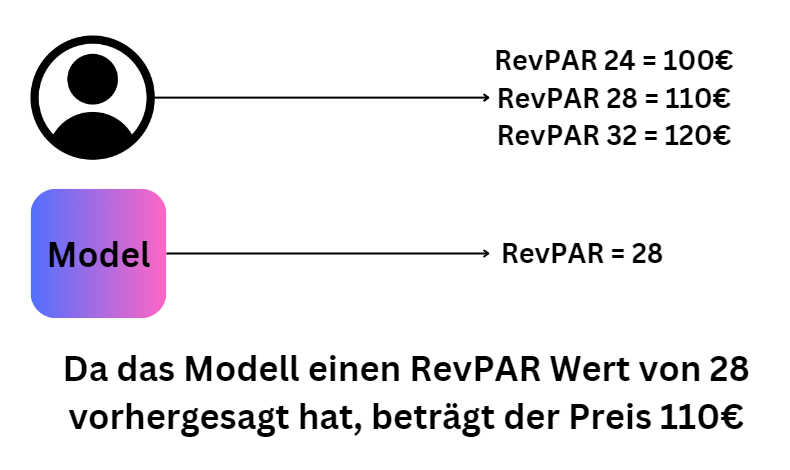
\includegraphics[width=0.5\textwidth, center]{RevPAR_all.png}
    \caption[RevPAR-Modell Vorgehen]{RevPAR-Modell Vorgehen}
    \label{img:all_hotels}
\end{figure}

Dieser Ansatz zielt darauf ab, eine umfassende Verwendung der vorhandenen Daten zu ermöglichen und somit auch für Hotels ohne historische Buchungsdaten eine Prognose des RevPAR auf der Grundlage ihrer individuellen Eigenschaften zu ermöglichen.
\section{Mitbewerber Modell}
\label{sec:Mitbewerber}
Die grundlegende Idee des Konzeptes: Mitbewerber Modell ist es, die Daten von der Konkurrenz zu benutzen um daraufhin Preisvorschläge zu generieren. 
\newline
\newline
Durch dritt Anbieter wie \emph{HQ-Revenue} können Konkurrenzdaten genutzt werden um ein Modell aufzubauen. HQ-Revenue ist ein Anbieter, welcher Internetseiten wie Bookings.com oder trivago \emph{scraped} um an Hotelpreise oder andere Daten zu kommen. Dabei gibt es viele verschiedene Vorgehensweisen um Preise für ein Hotel ohne Vergangenheitsdaten zu entwickeln. Ein Primitiver Ansatz dabei wäre es, wenn alle Preise von den Konkurrenten genommen werden und damit der Durchschnitt ermittelt wird. Dies hat natürlich nichts mit Machine Learning oder geschweige denn Data Science zu tun aber es wäre ein Ansatz der Verfolgt werden könnte. 
\newline
\newline
Dieser Ansatz birgt jedoch eine Problematik: Nicht jeder Kunde von happyhotel hat auch automatisch Konkurrenzdaten zur Verfügung, diese müssen noch dazu gebucht werden. Deswegen wird folgender Ansatz verfolgt. 
\newline
\newline
So wie im vorherigen Konzept \emph{\nameref{sec:all_Hotels}} werden auch hier die Hotels in eine Vergleichbare Form gebracht. Das Ziel ist es dann ein oder mehrere Hotels zu finden, die vermeintlich ähnlich sind. Sobald ein oder mehrere ähnliche Hotels gefunden worden sind, können die Konkurrenzdaten von den ähnlichen Hotels genutzt werden. 
\newline
\newline
Als Zielvariable des Modells werden dann die Preise des ähnlichsten Hotels verwenden.  Jedoch sollen hierbei die Preise von den Konkurrenten und von dem ähnlichsten Hotel nicht einfach so benutzt werden, sondern lediglich das Verhältnis. Die Preise sollen anhand von dem Durchschnittlichen Preis in Verhältnis gebracht werden und dieses Verhältnis soll vorhergesagt werden. 
\newline
\newline 
Das Hotel ohne Vergangenheitsdaten muss in diesem Fall dann einen Durchschnittlichen Preise angeben, anhand dessen mit dem vorhergesagten  Verhältnis der tatsächliche Preis abgeleitet werden kann. Dies soll im folgenden Schaubild noch einmal dargestellt werden:
\begin{figure}[h]
    \centering
    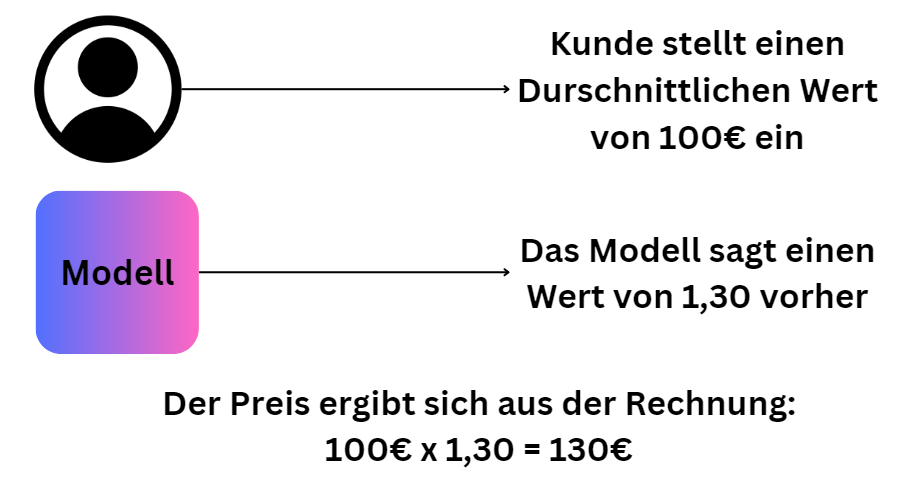
\includegraphics[width=0.5\textwidth, center]{Mitbewerber_model.png}
    \caption[Mitbewerber Modell]{Mitbewerber Modell}
    \label{img:all_hotels}
\end{figure}

\section{Ähnliche Hotels}
\label{sec:aehnliche_hotels}
Dieses Konzept der \emph{Ähnlichen Hotels} verschmilzt in gewisser Weise die Ideen der beiden Konzepte \emph{Mitbewerber Modell} und \emph{Hotel Daten von vielen Hotels}. Dieser Ansatz zielt darauf ab, ähnliche Hotels zu identifizieren und basierend auf den Daten dieser Hotels ein Modell zu entwickeln.
\newline
\newline
Im Gegensatz zum Konzept \emph{Hotel Daten von vielen Hotels} besteht bei diesem Ansatz die Möglichkeit, konkrete Buchungsdaten der jeweiligen Hotels zu verwenden. Die primäre Herausforderung liegt jedoch darin, die ähnlichsten Hotels zu identifizieren. Nachdem diese ähnlichen Hotels ausfindig gemacht wurden, kann das bereits vorhandene Modell \emph{Kombination aus RevPAR und Buchungskurve} ohne jegliche Anpassungen genutzt werden.
\newline
\newline
Dieses Modell wird dann, ähnlich wie bei anderen Hotels, mit den Buchungsdaten der zugrunde liegenden ähnlichen Hotels gefüttert, um Preise zu generieren. In diesem Szenario muss der Kunde lediglich eine Zuordnung zwischen dem RevPAR-Wert und dem konkreten Preis des Hotels festlegen.
\newline
\newline
Diese Vorgehensweise kombiniert die Vorteile beider vorherigen Konzepte, indem er sowohl auf die Ähnlichkeitsfindung zwischen Hotels, als auch auf die Nutzung spezifischer Buchungsdaten abzielt. Durch die Verwendung vorhandener Modelle ohne umfangreiche Modifikationen können so gezielt Preisvorhersagen für ähnliche Hotels generiert werden.
\section{Synthetische Daten erstellen}
\label{sec:Synthetische}
Das Konzept der \emph{Erstellung synthetischer Daten} markiert einen innovativen Ansatz innerhalb der Konzepte und weicht von den bisherigen Strategien ab. Dieser Ansatz verfolgt die Idee, ein Modell mit sämtlichen verfügbaren Daten zu trainieren und darauf aufbauend synthetische zukünftige Daten zu generieren. Ziel ist es, eine Art Simulation zu erstellen, die den Buchungsverlauf eines Hotels nachbildet.
\newline
\newline
Mittels dieser Simulation wird angestrebt, Vorhersagen darüber zu treffen, wie viele Buchungen für bestimmte Zimmerkategorien an bestimmten Tagen eingehen werden. Dadurch soll die Möglichkeit geschaffen werden, einen dynamischen Preis entsprechend dem erwarteten Buchungsverlauf zu gestalten.
\newline
\newline
Die Grundidee hinter dieser Vorgehensweise liegt in der Schaffung eines virtuellen Modells, welches basierend auf vergangenen Daten und Mustern potenzielle zukünftige Buchungen simuliert. Hierbei sollen verschiedene Szenarien durchgespielt werden, um die wahrscheinlichsten Buchungstrends abzuschätzen, und somit einen fundierten Ansatz für die dynamische Preisgestaltung zu generieren.
\section{Evaluation}
\label{sec:eval_konzept}
Nachdem nun die ausgearbeiteten Konzepte vorgestellt wurden, gilt es diese zu Bewerten um festzulegen mit welchen Konzepten fortgefahren werden soll. Jedes der vorgestellten ist auf seine Art valide und hat auch Berechtigung verfolgt zu werden. Um deshalb entscheiden zu können, welches Konzept überhaupt nachgegangen werden soll oder in welcher Reihenfolge die Konzepte ausprobiert werden sollen, werden die Konzepte nach den folgenden Kriterien bewertet:
\begin{itemize}
    \item Aufwand
    \item Erfolgswahrscheinlichkeit
    \item Impact
\end{itemize}
Aufwand und Erfolgswahrscheinlichkeit sind selbsterklärend. Der Impact bezieht sich darauf, in wie fern happyhotel im generellen von dem Konzept profitieren könnte und ob das Konzept nicht auch für schon vorhandene Kunden eingesetzt werden könnte.
\newline
\newline
Jedes Konzept kann bei jedem Kriterium eine Zahl zwischen 1 bis 5 erzielen, wobei 5 das Beste und 1 das Schlechteste in dem jeweiligen Kriterium bedeutet. Die Ergebnisse der Evaluation sind wie folgt in der Tabelle dargestellt:
\begin{table}[ht]
    \centering
    \begin{tabularx}{\textwidth}{|d|c|c|c|c|}
        \textbf{Konzepte} & \textbf{Aufwand} & \textbf{Erfolgsw.} & \textbf{Impact} & \textbf{Result} \\
        \hline
        Daten von vielen Hotels & 4       & 4            & 4      & 12 
        \\\rowcolor{Gray}
        Mitbewerber             & 4       & 3            & 3      & 10                \\
        Ähnliche Hotels         & 4       & 5            & 4      & 13  
        \\\rowcolor{Gray}
        Synthetischen Daten     & 1       & 3            & 5      & 9   \\
    \end{tabularx}
    \caption[Evaluierung der Konzepte]{Evaluierung der Konzepte}
    \label{table:eval_kozepts}
\end{table}

Nach der Evaluierung wurde bestimmt, dass das Konzept \emph{\nameref{sec:aehnliche_hotels}} das größte Potenzial hat und soll dementsprechend auch verfolgt werden. Je nach Zeit und Ergebnisse werden die Konzepte \emph{\nameref{sec:Mitbewerber}} und \emph{\nameref{sec:all_Hotels}} auch verfolgt und evaluiert werden. Die Erstellung einer Simulation durch Synthetische Daten ist auch ein sehr interessantes Konzept, würde aber im rahmen dieser Thesis zu weit gehen.
\chapter{Ähnliche Hotels}
\label{chap:Similar_hotels}
Die Evaluierung der verschiedenen Konzepte, wie sie im vorangegangenen Kapitel \emph{\nameref{chap:konzepte}} ausführlich dargelegt wurden, führte zu einer kritischen Entscheidung bezüglich des anfänglichen Fokus für die strategische Ausrichtung. Nach einer umfassenden Analyse und Bewertung wurde klar, dass das Konzept der \emph{\nameref{sec:aehnliche_hotels}} sich als überzeugende und vielversprechende Lösung für das vorliegende Problem erweist.
\newline
\newline
Dieses Kapitel konzentriert sich daher detailliert auf das Konzept der \emph{\nameref{sec:aehnliche_hotels}}. Es zielt darauf ab, die spezifische Methodik und Herangehensweise dieses Konzepts zu beleuchten. Die kommenden Abschnitte bieten eine eingehende Analyse, die durch umfassende Datenanalysen und Experimente unterstützt wird. Dadurch soll ein tiefgreifendes Verständnis für die erfolgreiche Umsetzung des Konzepts der \emph{\nameref{sec:aehnliche_hotels}} vermittelt werden.
\newline
\newline
Wie in der Sektion \emph{\nameref{sec:aehnliche_hotels}} beschrieben, liegt der Fokus zunächst darauf, ähnliche Hotels zu identifizieren, die als Grundlage für die Anpassung und Anwendung des bereits bestehenden RevPAR-Modells dienen sollen.

\section{Finden von ähnlichen Hotels}
\label{sec:find_similar}
Das Finden von ähnlichen Hotels ist die Grundlage dieses Konzeptes. Um dies zu erreichen, soll das Vorgehen, welches in der Sektion \emph{\nameref{sec:aehnliche_hotels}} beschrieben wurde, verfolgt werden. Angefangen mit der Datenbeschaffung, muss sich zunächst ein Überblick darüber gemacht werden, welche Daten schon vorhanden sind und welche Daten gegebenfalls noch besorgt werden müssen, bevor dann mit der Datenanalyse und der Modellierung weiter gemacht werden kann. 

\subsection{Datenbeschaffung}
\label{subsec:Datenbeschaffung}
Durch die verschiedenen Property Management Systeme sind für die einzelnen Hotels bereits Stammdaten wie Zimmeranzahl oder Zimmerkategorien vorhanden. Zudem wird der jeweilige Kunde beim Einrichten von happyhotel auch schon nach verschiedenen Daten befragt. Unter den Daten, die bei einem Kunden abgefragt werden, gehören Informationen wie zum Beispiel die Adresse des jeweiligen Hotels. 
\newline
\newline
Werden nun alle schon vorhanden Informationen zusammengetragen, die bisher in der Datenbank zur Verfügung stehen, entsteht dabei das folgende Dataframe:
\begin{figure}[h]
    \centering
    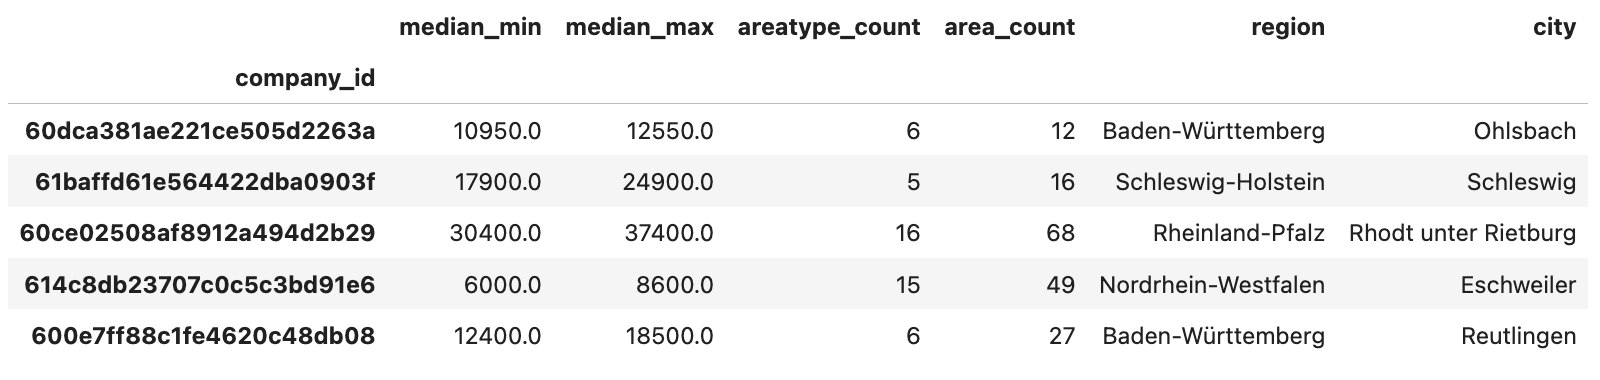
\includegraphics[width=1\textwidth, center]{Features_1.png}
    \caption[Alle schon vorhanden Features]{Alle schon vorhanden Features}
    \label{img:all_Features}
\end{figure}

In Abbildung \ref{img:all_Features} sind die Daten zu sehen, die bislang zur Verfügung stehen, wobei sich die \emph{median\_min} und \emph{median\_max} Werte auf den Median aller Zimmerkategorie-Preise bezieht.
\newline
\newline
Dadurch, dass \emph{region} und \emph{city} manuell vom Kunden eingetragene Werte sind, ergab sich eine gewisse Skepsis, ob alle Werte norm-konform eingetragen wurden. Aufgrund dieser Skepsis sollte eine kleine Datenanalyse getätigt werden. 
\newline
\newline
Bei der Datenanalyse wurde jeweils nach der Region und nach der Stadt gruppiert, um zu prüfen ob die Daten so benutzt werden können. Im Folgenden sind die Werte jeweils für die Region und für die Stadt zu sehen:

\begin{figure}[h]
    \centering
    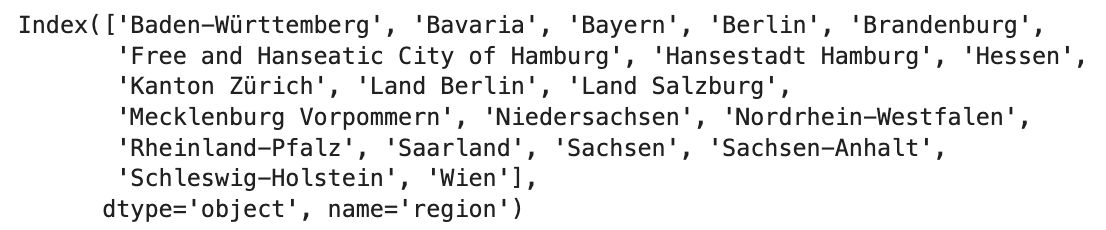
\includegraphics[width=0.8\textwidth, center]{region_1.png}
    \caption[Alle vorhanden Regionen]{Alle vorhanden Regionen}
    \label{img:region_1}
\end{figure}

\begin{figure}[h]
    \centering
    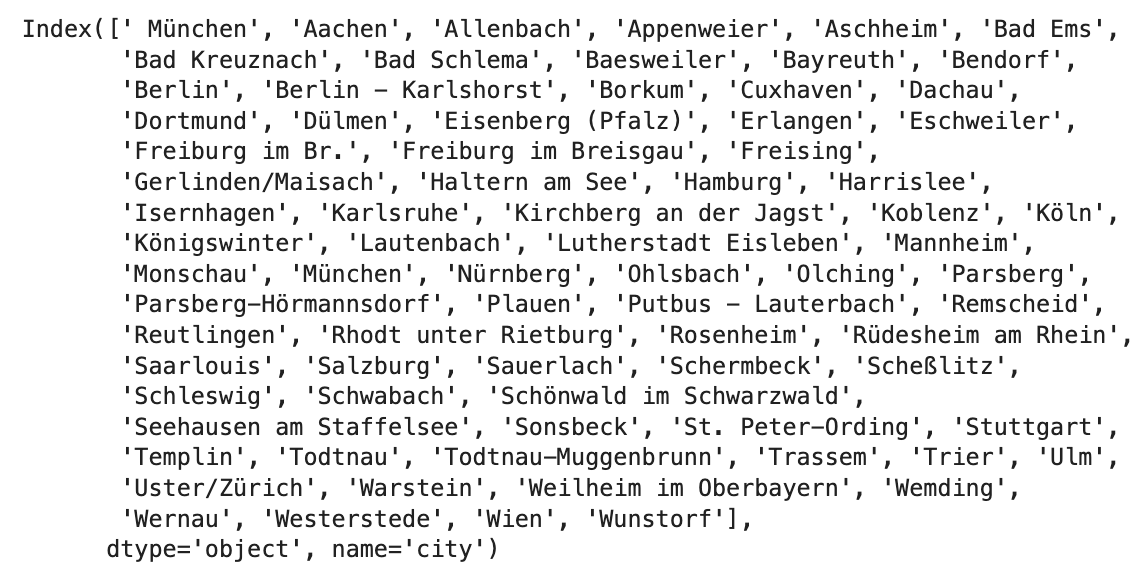
\includegraphics[width=0.8\textwidth, center]{city_1.png}
    \caption[Alle vorhanden Städte]{Alle vorhanden Städte}
    \label{img:city_1}
\end{figure}

Es ist eindeutig zu erkennen, dass es sowohl bei der Region als auch bei der Stadt zu einer Inkonsistenz kommt. So wurde die Region \emph{Berlin} sowohl als \emph{Berlin}, als auch mit \emph{Land Berlin} angegeben. Auch bei der Stadt ist die Diskrepanz deutlich zu erkennen, -so wurde bspw. \emph{München} mit Leerzeichen vorne dran angegeben oder die Stadt Freiburg einmal mit der Abkürzung \emph{Br.} und ein anderes Mal mit komplett ausgeschriebenen \emph{Breisgau} angegeben. Es ergab sich also, dass diese Werte so wie sie sind, nicht verwendet werden können.

\input{kapitel/Similar_Hotels/sections/subsections/Beschaffung_1.tex}
\input{kapitel/Similar_Hotels/sections/subsections/Beschaffung_2.tex}
\subsection{Datenvorverarbeitung}
\label{subsec:Datenvorverarbeitung}
Nach der Datenbeschaffung erfolgt die Datenvorverarbeitung, die darauf abzielt, die Qualität und Integrität der Daten sicherzustellen. Ein zentraler Schwerpunkt liegt dabei auf der Identifikation und Eliminierung fehlerhafter oder ungültiger Datensätze. Häufig wird innerhalb der Datensätze nach Nullwerten gesucht, um diese entweder durch valide Daten zu ersetzen oder in einigen Fällen gänzlich zu entfernen. Im vorliegenden Fall ist es Wichtig, dass sämtliche als verwendbar gekennzeichneten Hotels in die Analyse einbezogen werden. Die Datensätze sollen nicht einfach verworfen werden; vielmehr erfolgt eine gezielte Substitution von Nullwerten durch valide Daten, um eine konsistente und zuverlässige Grundlage für die weiterführende Analyse zu gewährleisten \cite{Agarwal.05.10.2018}.
\newline
\newline
Im folgenden ist die Anzahl aller Nullwerte innerhalb des Datensatzes zu sehen:
\begin{figure}[h]
    \centering
    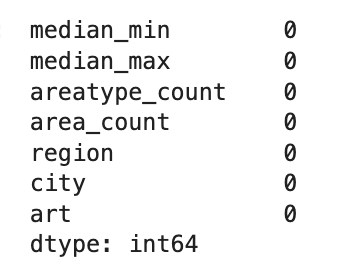
\includegraphics[width=0.4\textwidth, center]{Null_values.png}
    \caption[Summe aller Nullwerte im Datensatz]{Summe aller Nullwerte im Datensatz}
    \label{img:null_values}
\end{figure}

In Abbildung \ref{img:null_values} ist zu sehen, dass innerhalb des es Datensatzes keine Nullwerte gibt und somit auch keine Datenvorverarbeitung getätigt werden muss.
\subsection{Allgemeine Datenanalyse}
\label{subsec:Datenanalyse}
Die Datenanalyse ist ein, wenn nicht sogar der Wichtigste schritt im Data Science Bereich \cite{Agarwal.05.10.2018}. Dabei sollen die Daten ergründet und verstanden werden. Dieser Schritt soll nicht nur ein Verständnis für die vorliegenden Daten schaffen, sondern auch \emph{outlier} erfassen. Meist wird auch versucht innerhalb der Datenanalyse zusammenhänge zu der Zielvariable zu finden. Dies setzt jedoch voraus, dass eine Zielvariable vorhanden ist. In dem vorliegenden Fall existiert keine Zielvariable, da nicht bekannt ist welche Hotels mit welchen Hotels ähnlich sind. Aufgrund dessen, dass keine Zielvariable vorhanden ist, wird die folgende Datenanalyse lediglich dazu genutzt um die Daten besser zu verstehen. Zudem soll festgestellt werden, welche Daten wie als Features verwendet werden können.
\newline
\newline
Für die Datenanalyse soll die Python-Bibliothek \emph{Seaborn} benutzt werden. Die \emph{Seaborn}-Bibliothek stellt ein leistungsstarkes Werkzeug dar, das speziell für die Erstellung von statistischen Grafiken in Python entwickelt wurde \cite{Melanie.2023}. Das Hauptziel besteht darin, die verschiedenen Verteilungen der Features auf anschauliche Weise darzustellen, um einen umfassenden Überblick über die zugrunde liegenden Daten zu ermöglichen. Durch die Nutzung der Funktionalitäten von \emph{Seaborn} wird eine effiziente und ästhetisch ansprechende Visualisierung erreicht, die es ermöglicht, Muster, Ausreißer oder Trends in den Daten leichter zu identifizieren.

\subsubsection{Region Features}
Zuallererst soll ein grober Überblick über die Städte der Hotels innerhalb der Datenbank erstellt werden. Dazu wird innerhalb des Datensatzes nach der Stadt um die Anzahl der Hotels einer Stadt zu ermitteln.

\newpage

\begin{figure}[h]
    \centering
    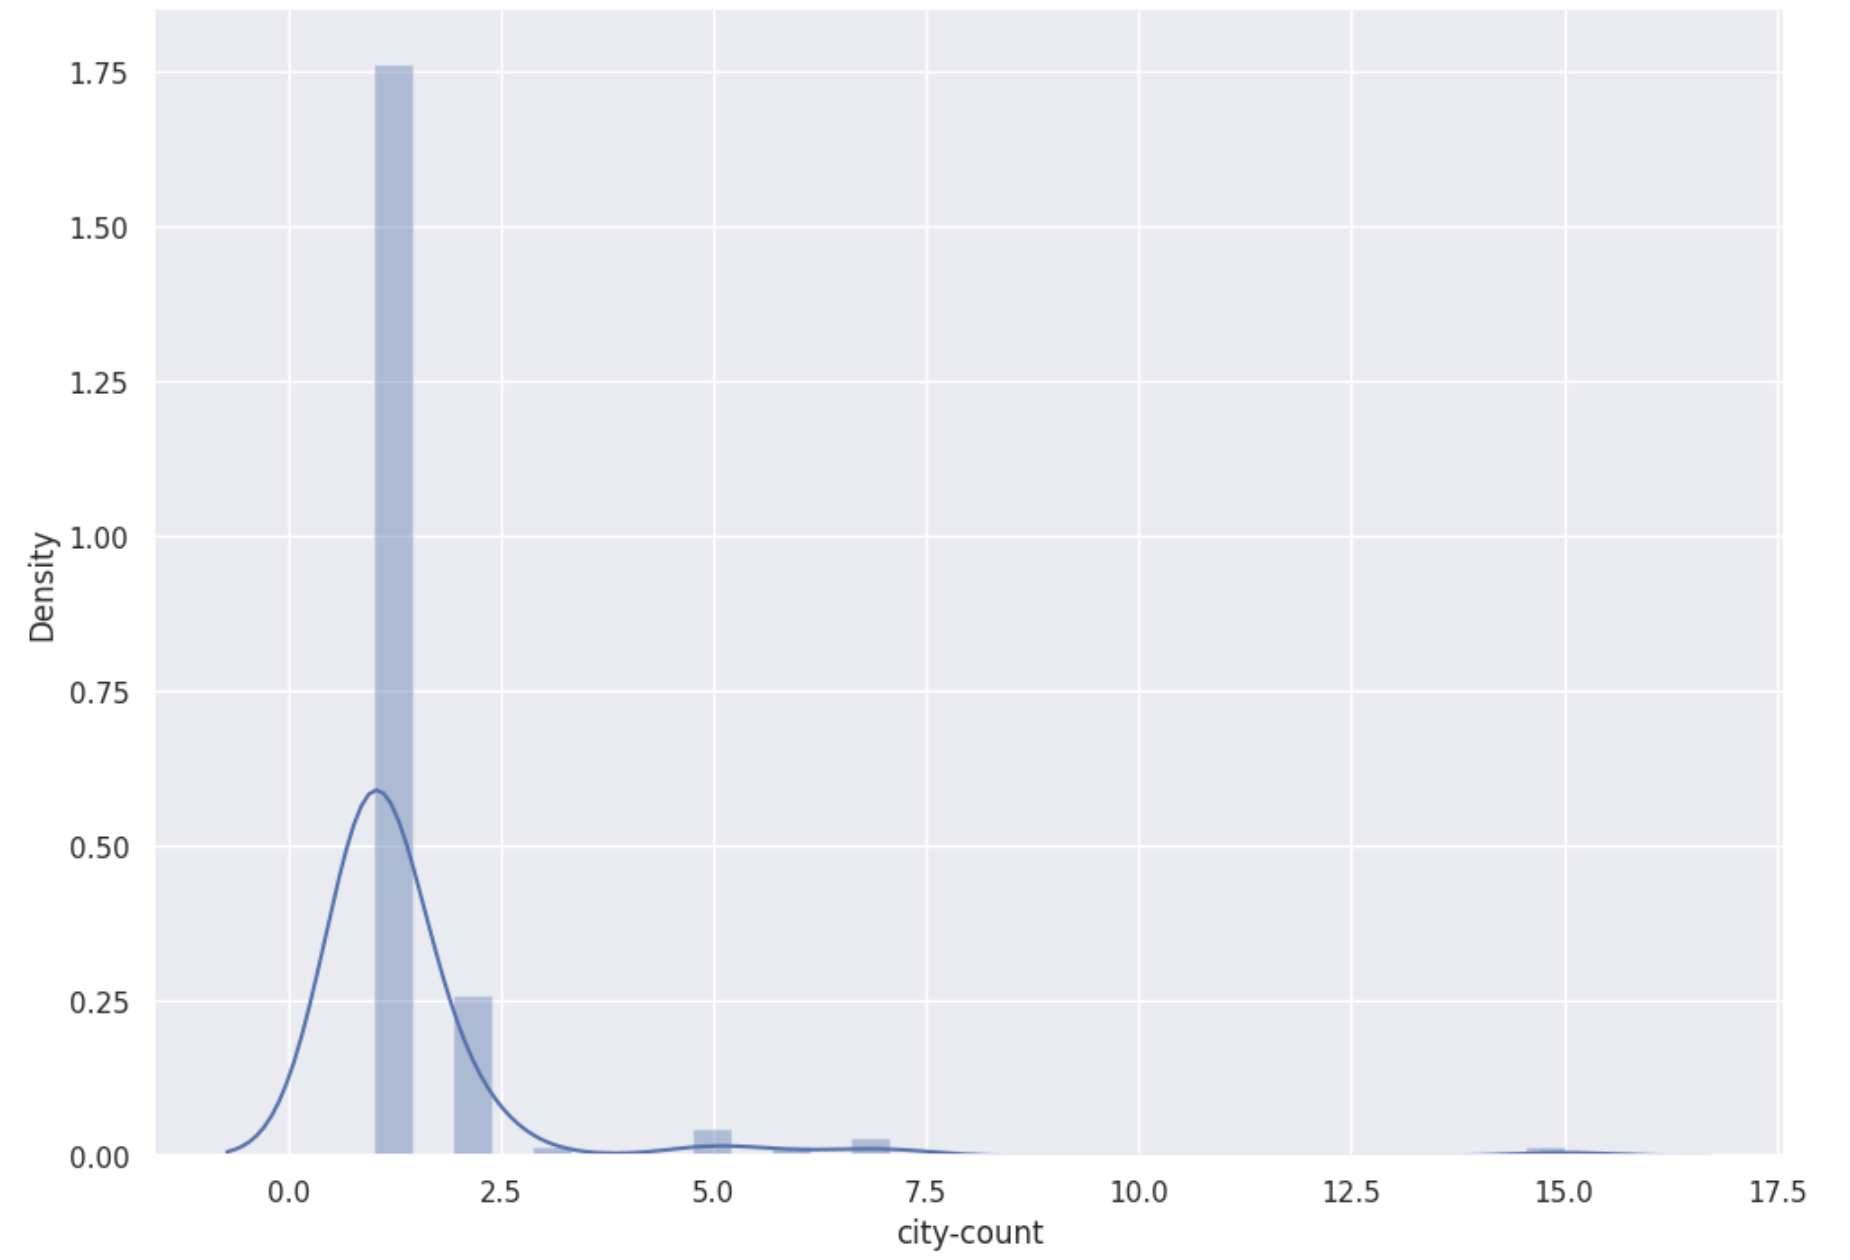
\includegraphics[width=1\textwidth, center]{verteilung_city.png}
    \caption[Verteilung der Städte]{Verteilung der Städte}
    \label{img:verteilung_city}
\end{figure}

Die Analyse der Abbildung \ref{img:verteilung_city} offenbart, dass die überwiegende Mehrheit der in der Datenbank erfassten Städte lediglich über ein einziges Hotel verfügt, welches happyhotel in Anspruch nimmt. Zugleich verdeutlicht die Abbildung \ref{img:verteilung_city}, dass es lediglich einen geringen Anteil von Städten gibt, in denen fünf oder mehr Hotels registriert sind. Dies ist etwas problematisch, da das Feature \emph{City} zu unausgewogen ist und so nicht mit in das Modell gegeben werden kann. Es muss also in einer anderen Form verwendet werden.
\newline
\newline
Momentan werden, wie in der Abbildung \ref{img:all_Features_2} gezeigt, die Stadt und die Region als zwei separate Features aufgelistet. Die Idee ist es nun die zwei Features zu verschmelzen und die Hotels in Regionen aufzuteilen um mehr Informationen zu erhalten. Anstatt also Region und Stadt separat zu haben soll es ein Feature Region geben, welches wie folgt aufgebaut ist: 

\begin{itemize}
    \item Befindet sich innerhalb einer Stadt Fünf oder mehr Hotels, so wird die Stadt ohne jegliche Modifikation als Region genommen.
    \item Befindet sich innerhalb einer Stadt weniger als Fünf Hotels, so setzt sich die Region aus der ursprünglichen Region, also dem Bundesland und der Größe der Stadt zusammen nach dem Schema: {Region}-{Größe}
\end{itemize}

Für die Idee muss zunächst ermittelt werden, in welchen Städte sich Fünf oder mehr Hotels befinden. Auch diese Information kann wie folgt Visualisiert werden:

\begin{figure}[h]
    \centering
    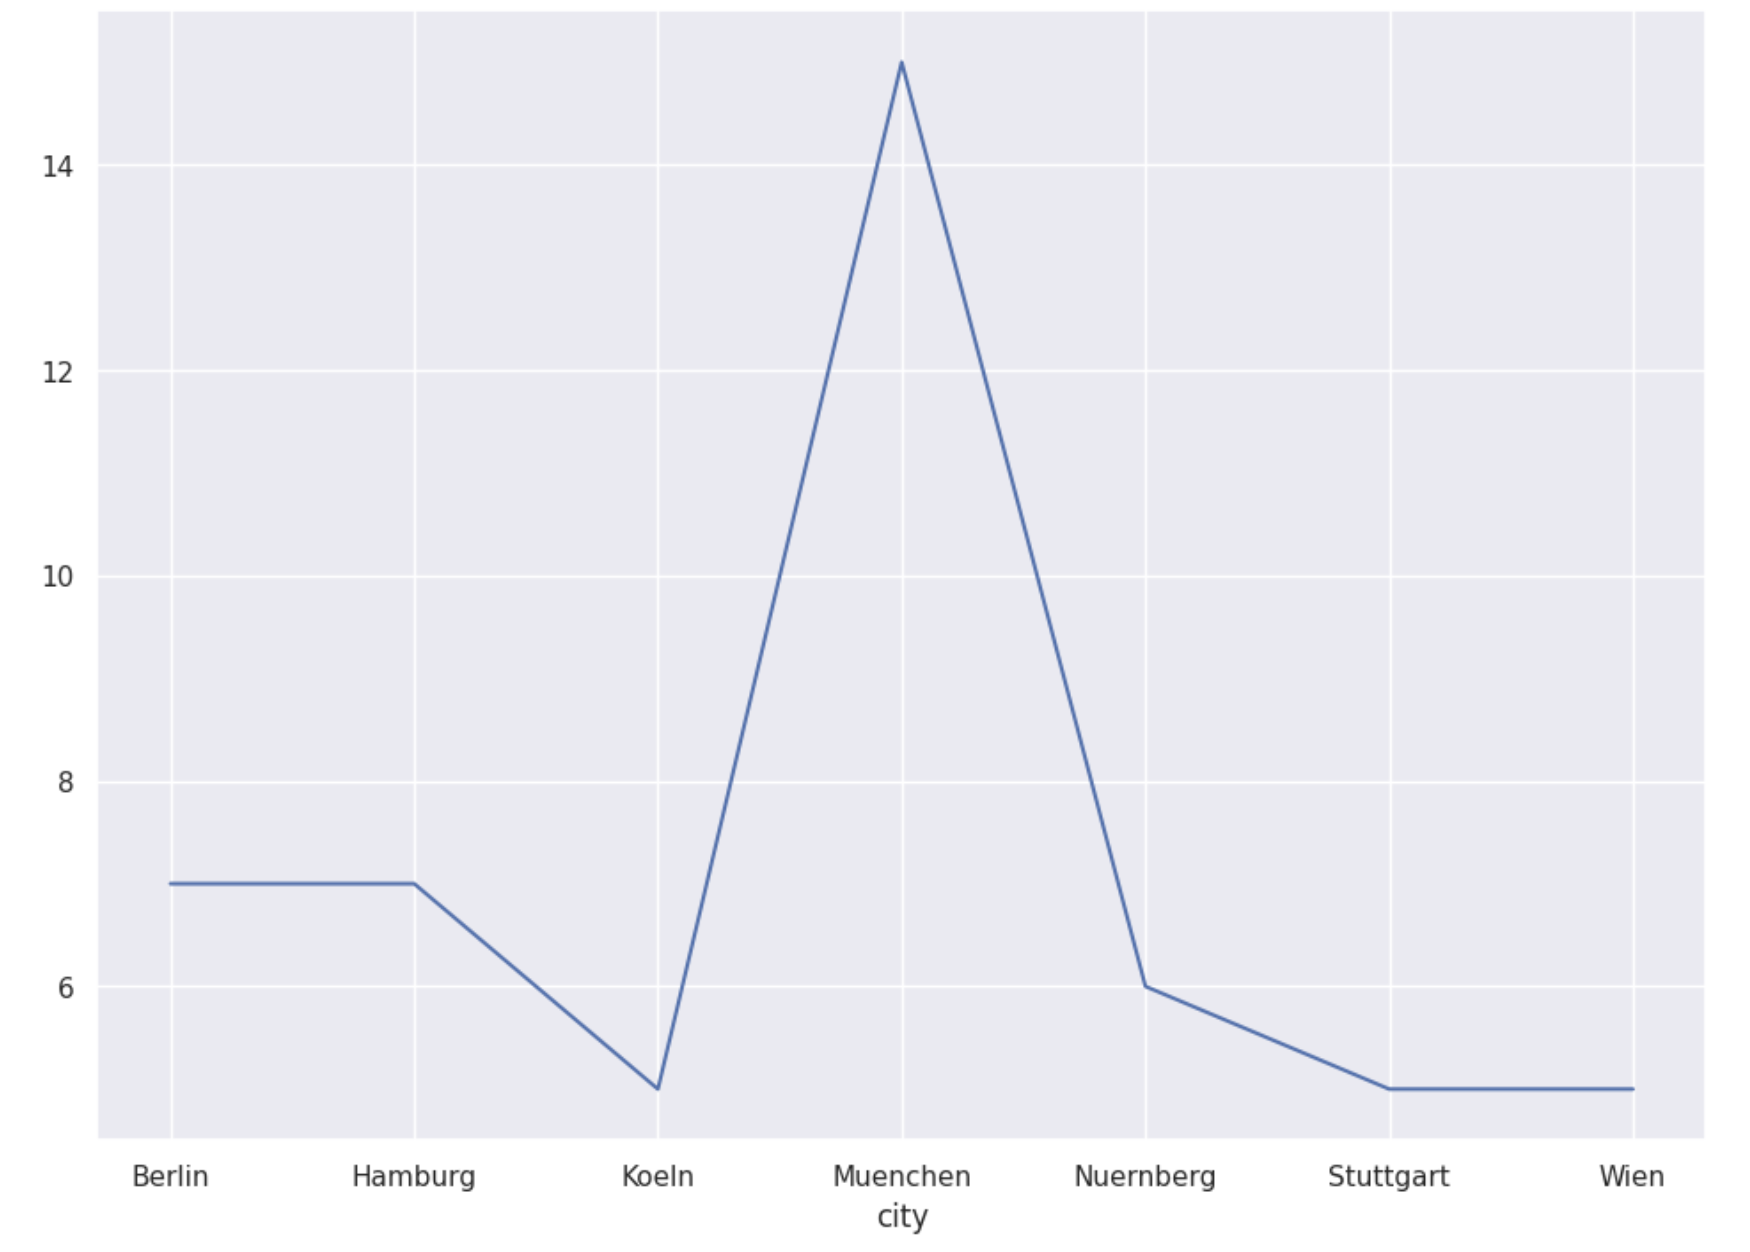
\includegraphics[width=1\textwidth, center]{city_five_or_more.png}
    \caption[Städte mit Fünf oder mehr Hotels]{Städte mit Fünf oder mehr Hotels}
    \label{img:city_five_or_more}
\end{figure}

Ganz klar zu erkennen ist, dass die Sieben Städte Berlin, Hamburg, Köln, München, Nürnberg, Stuttgart, und Wien die Städte sind, in denen Fünf oder mehr Hotels vorhanden sind. Die aufgelisteten Städte können dementsprechend so übernommen werden und für alle anderen wird die Regel von oben angewandt.
\newline
Nach der Umformulierung von Region und Stadt sieht der Datensatz wie folgt aus:

\begin{figure}[h]
    \centering
    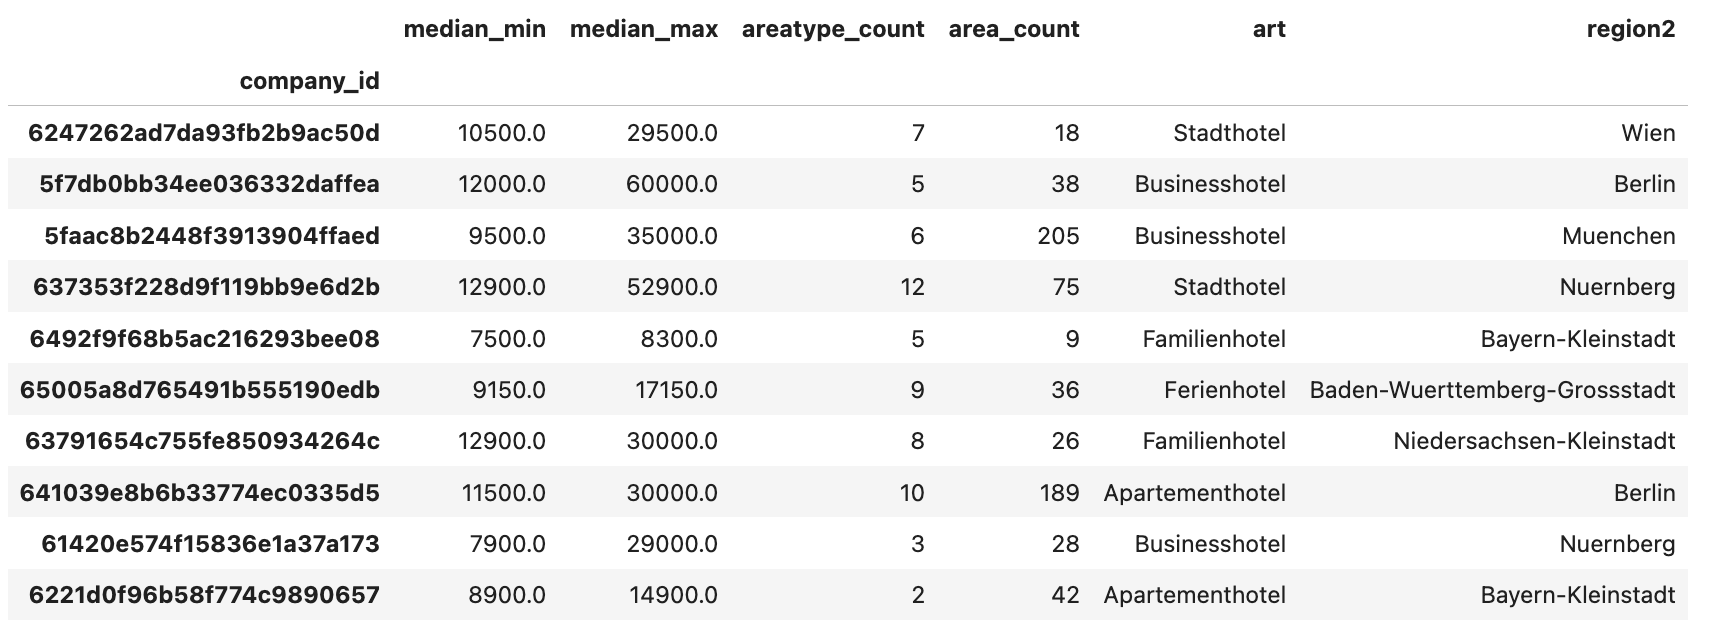
\includegraphics[width=1\textwidth, center]{all_features_3.png}
    \caption[Datensatz nach der Umformulierung]{Datensatz nach der Umformulierung}
    \label{img:all_features_3}
\end{figure}

Auch hier soll wieder die Verteilung visualisiert werden

\begin{figure}[h]
    \centering
    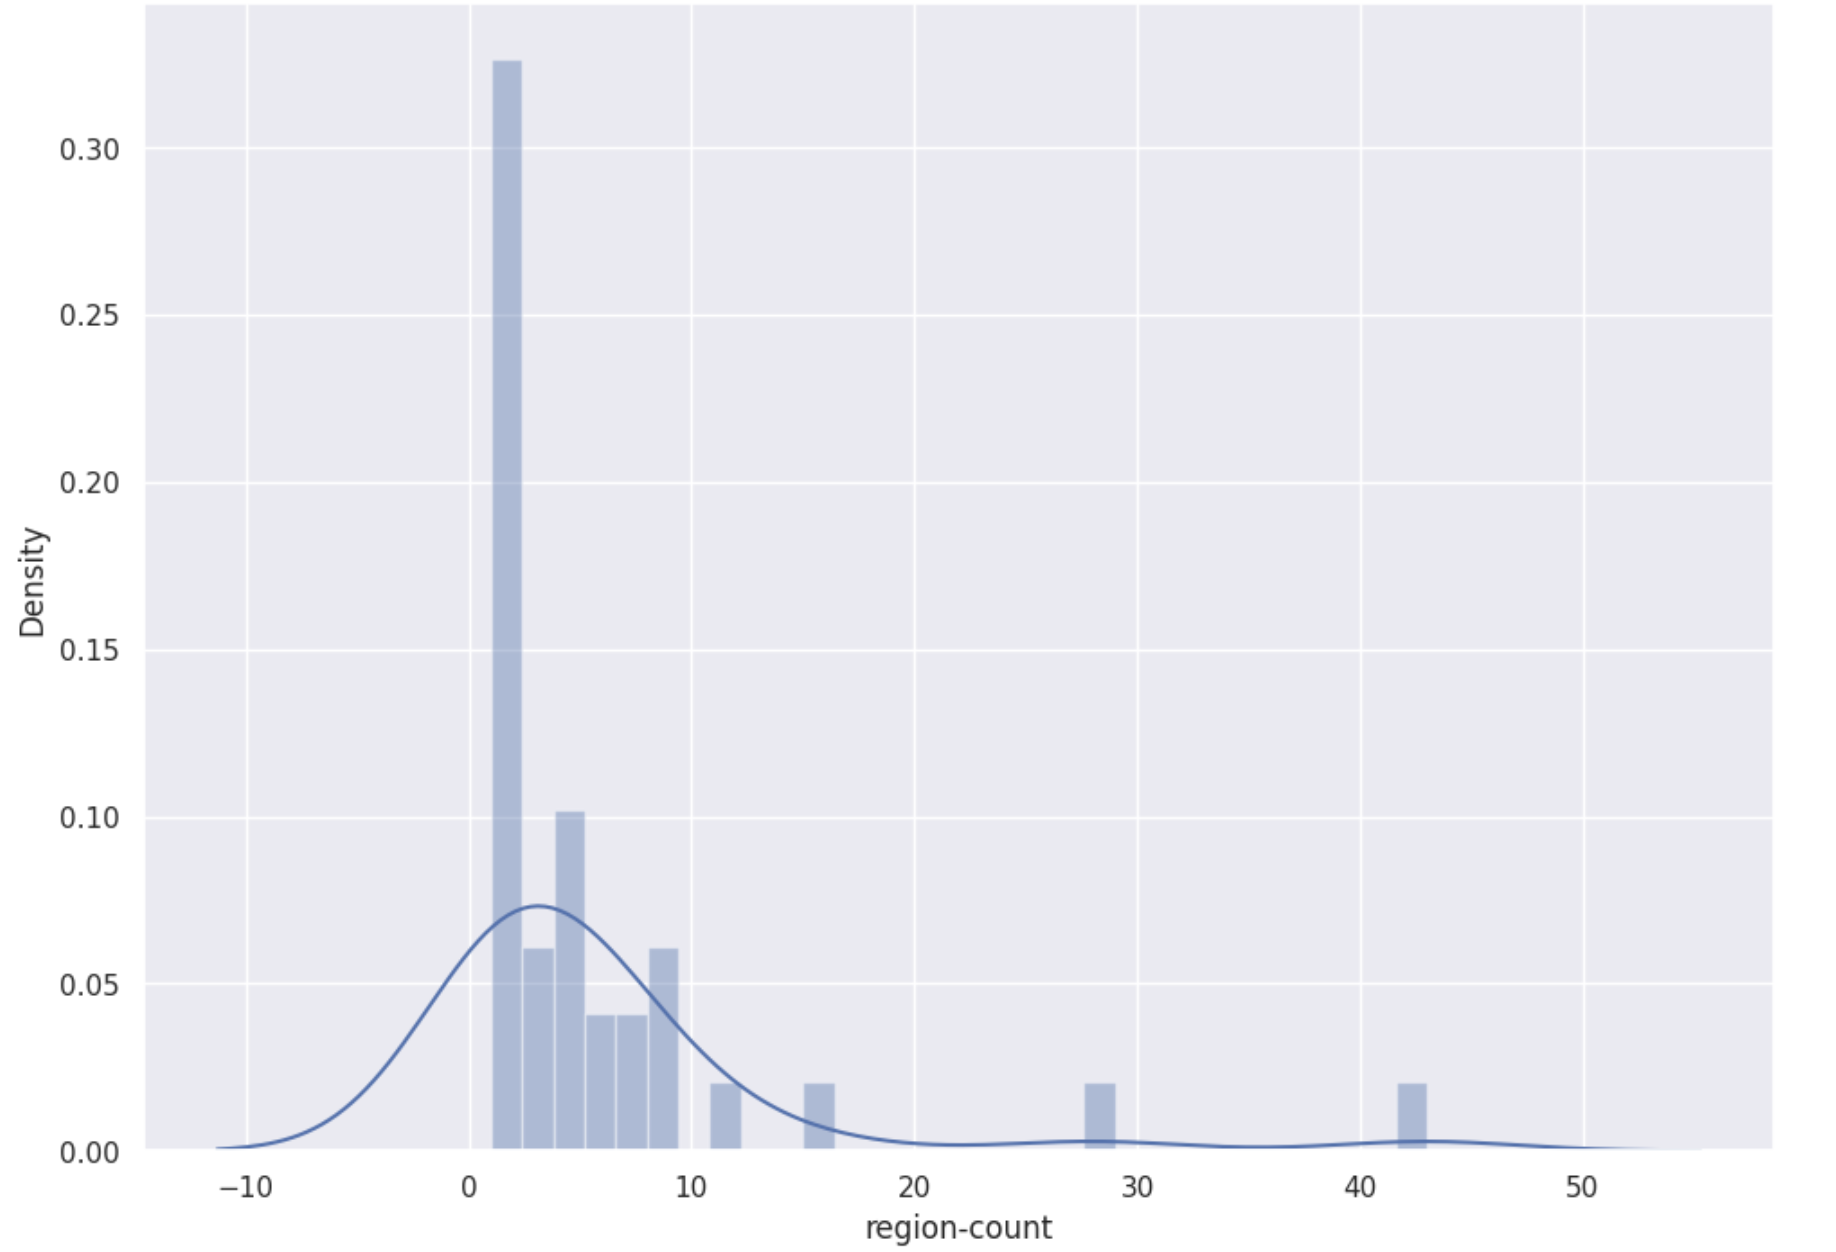
\includegraphics[width=1\textwidth, center]{verteilung_region2.png}
    \caption[Verteilung des neuen Features \emph{region2}]{Verteilung des neuen Features \emph{region2}}
    \label{img:verteilung_region_2}
\end{figure}

Es zeigt sich, dass noch immer ein großer Anteil des Datensatzes niedrigeren Bereich sich befindet, jedoch konnte mit der Modifikation ein bisschen mehr Varianz in die Daten gebracht werden.

\subsubsection{Preis Features}
Als nächstes sollen die Preis Features, namentlich betitelt mit \emph{median\_min} und \emph{median\_max}, erkundet und visualisiert werden. Hierzu soll wie auch bei der Region zunächst die Verteilung betrachtet werden:
\newpage
\begin{figure}[h]
    \centering
    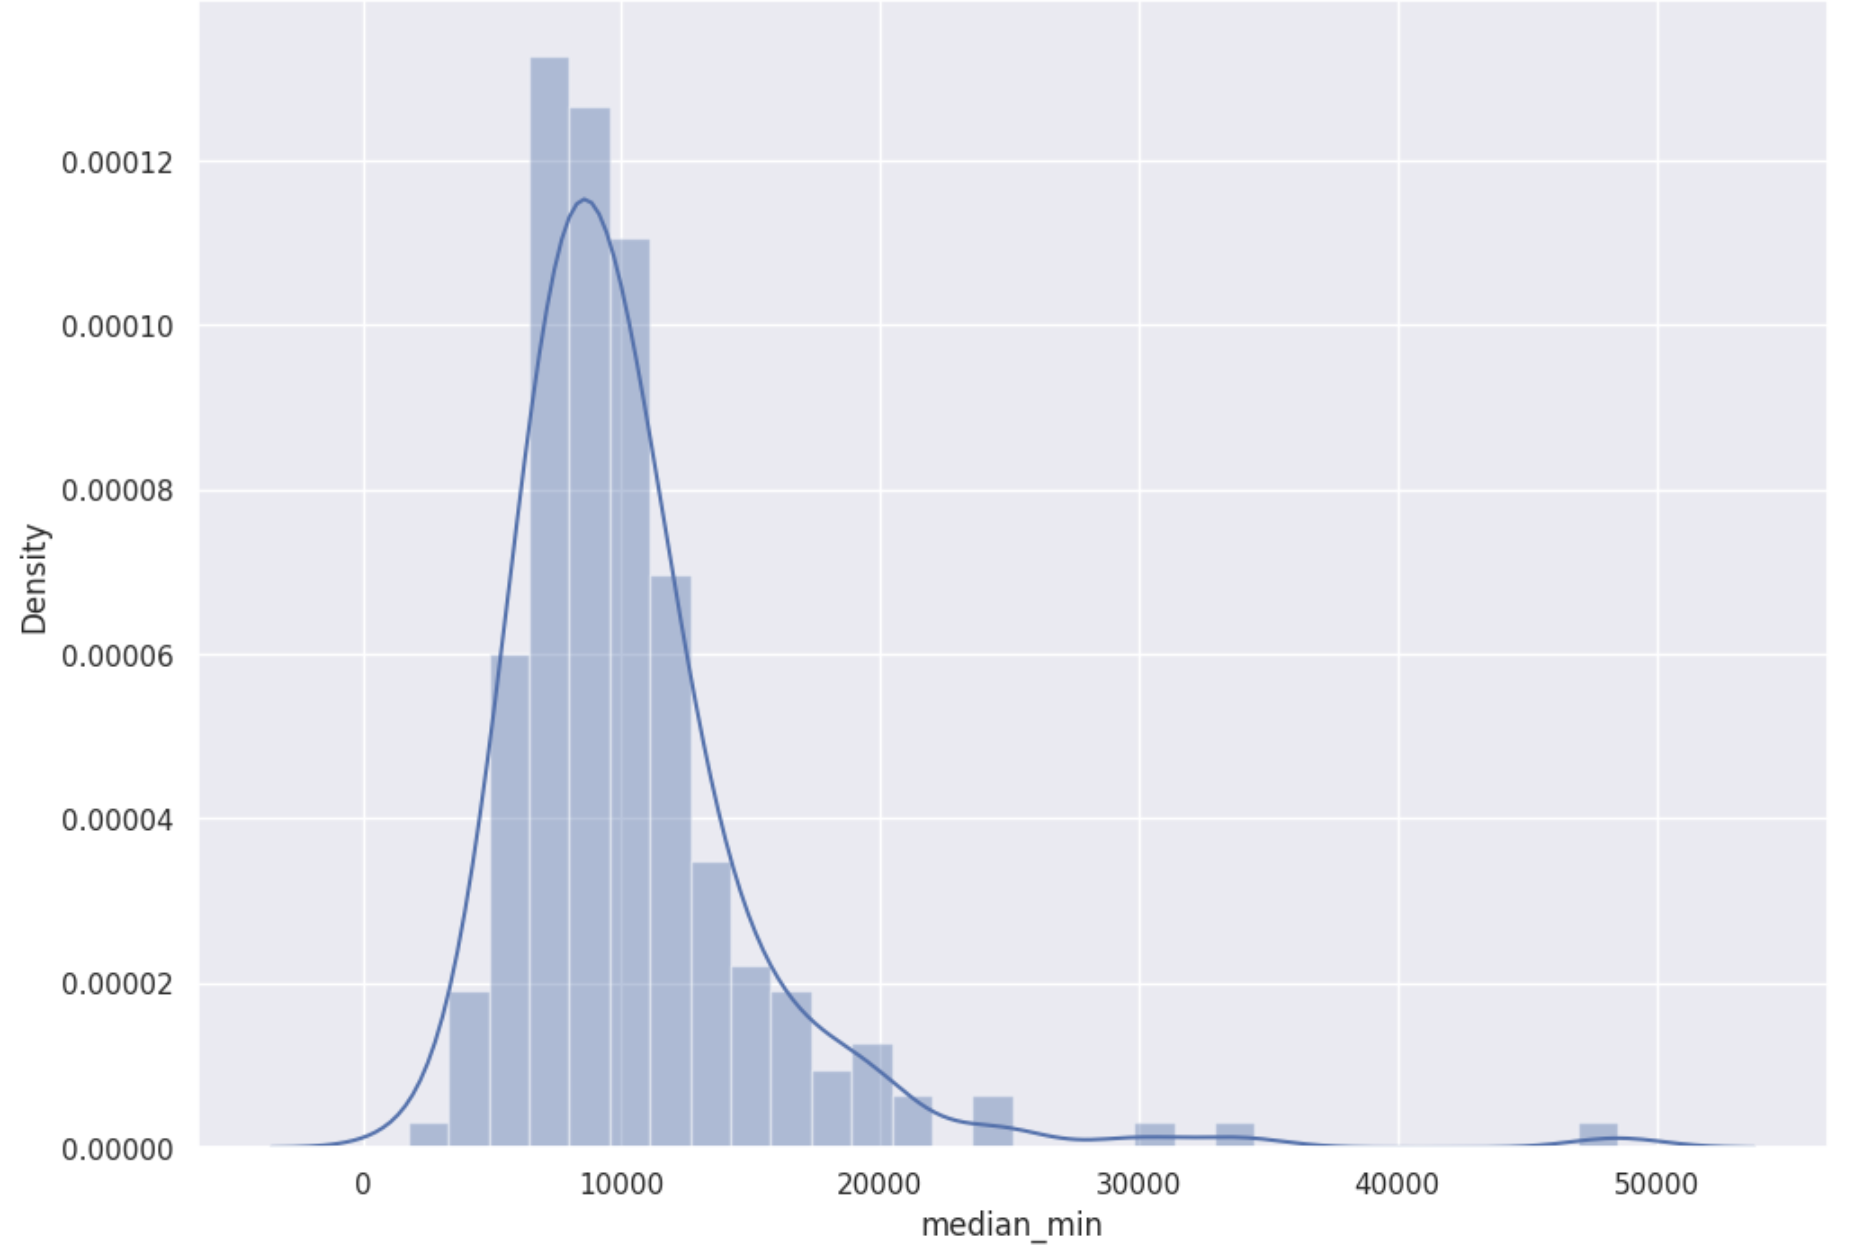
\includegraphics[width=1\textwidth, center]{verteilung_min.png}
    \caption[Verteilung von dem Preis Features \emph{median\_min}]{Verteilung von dem Preis Features \emph{median\_min}}
    \label{img:verteilung_min}
\end{figure}

Abbildung \ref{img:verteilung_min} zeigt, dass das Feature \emph{median\_min} eine Normalverteilung mit ein paar outlier aufweist. Eine Normalverteilung  sagt aus, dass die Verteilung mehr Daten um den Mittelwert herum aufweist. Die Datenverteilung nimmt ab, wenn sich vom Zentrum entfernt wird. Die resultierende Kurve ist symmetrisch zum Mittelwert und bildet eine glockenförmige Verteilung \cite{Shrishty.05.08.2021}.
\newline
\newline
Eine weitere interessante Information die noch aus dem Feature \emph{median\_min} gelesen werden kann, ist der Durchschnittliche Wert Region. Dazu soll der Datensatz nach der Region gruppiert werden und den Durchschnittlichen Wert ermittelt werden.
\newpage
\begin{figure}[h]
    \centering
    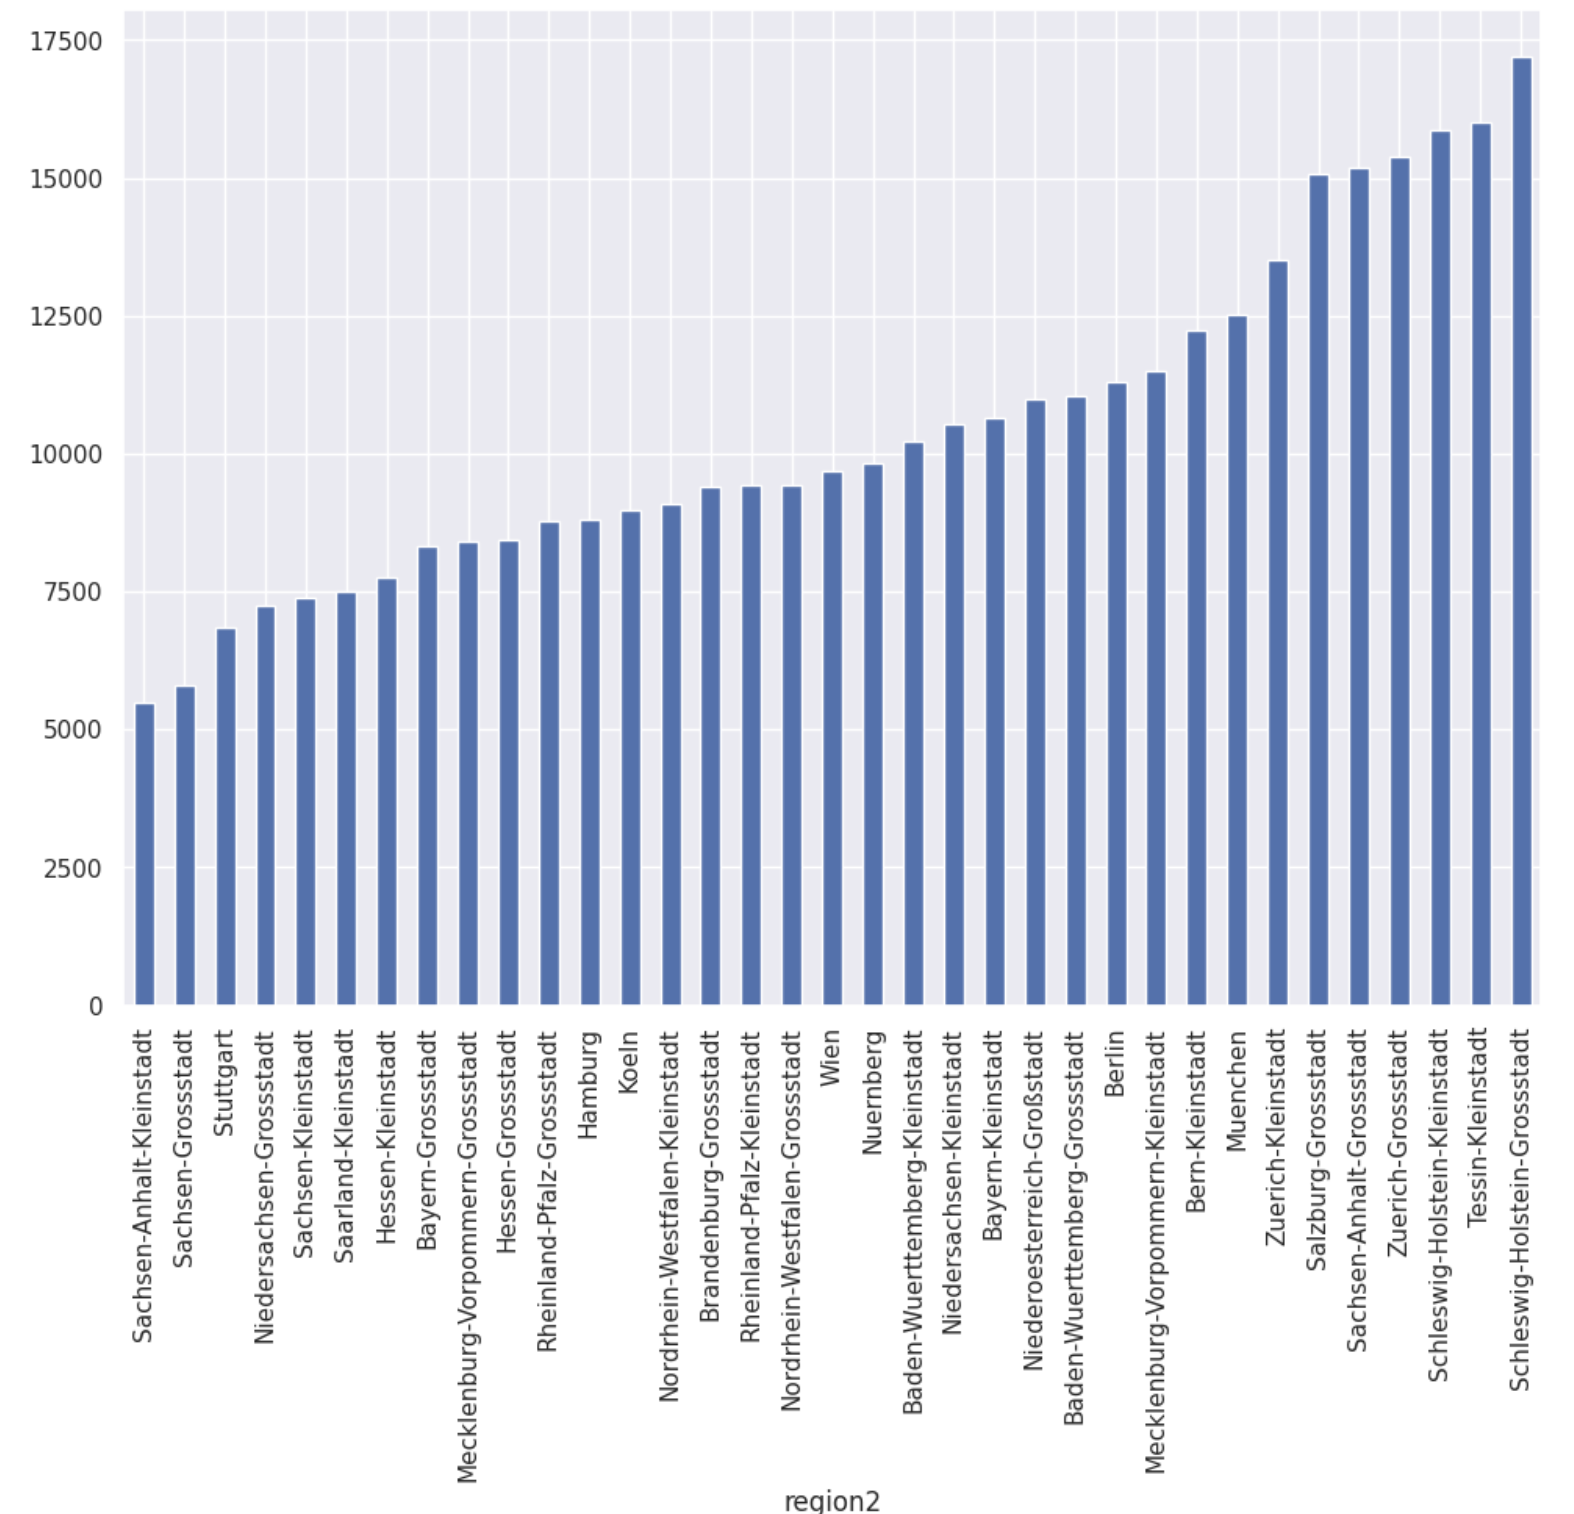
\includegraphics[width=0.6\textwidth, center]{avg_min_city.png}
    \caption[Durchschnittlicher minimal Preis pro Region]{Durchschnittlicher minimal Preis pro Region}
    \label{img:avg_min_city}
\end{figure}

Die Erkenntnis die aus der Abbildung \ref{img:avg_min_city} genommen werden kann, ist die, dass es einen deutlichen unterschied macht, in welcher Region das Hotel liegt wenn auf den Minimalen Median Preis des Hotel geschaut wird. Das gleich kann auch mit dem Maximalen Median Preis eines Hotels gemacht werden. Auch hier soll sich zunächst die Verteilung visualisiert werden:

\begin{figure}[h]
    \centering
    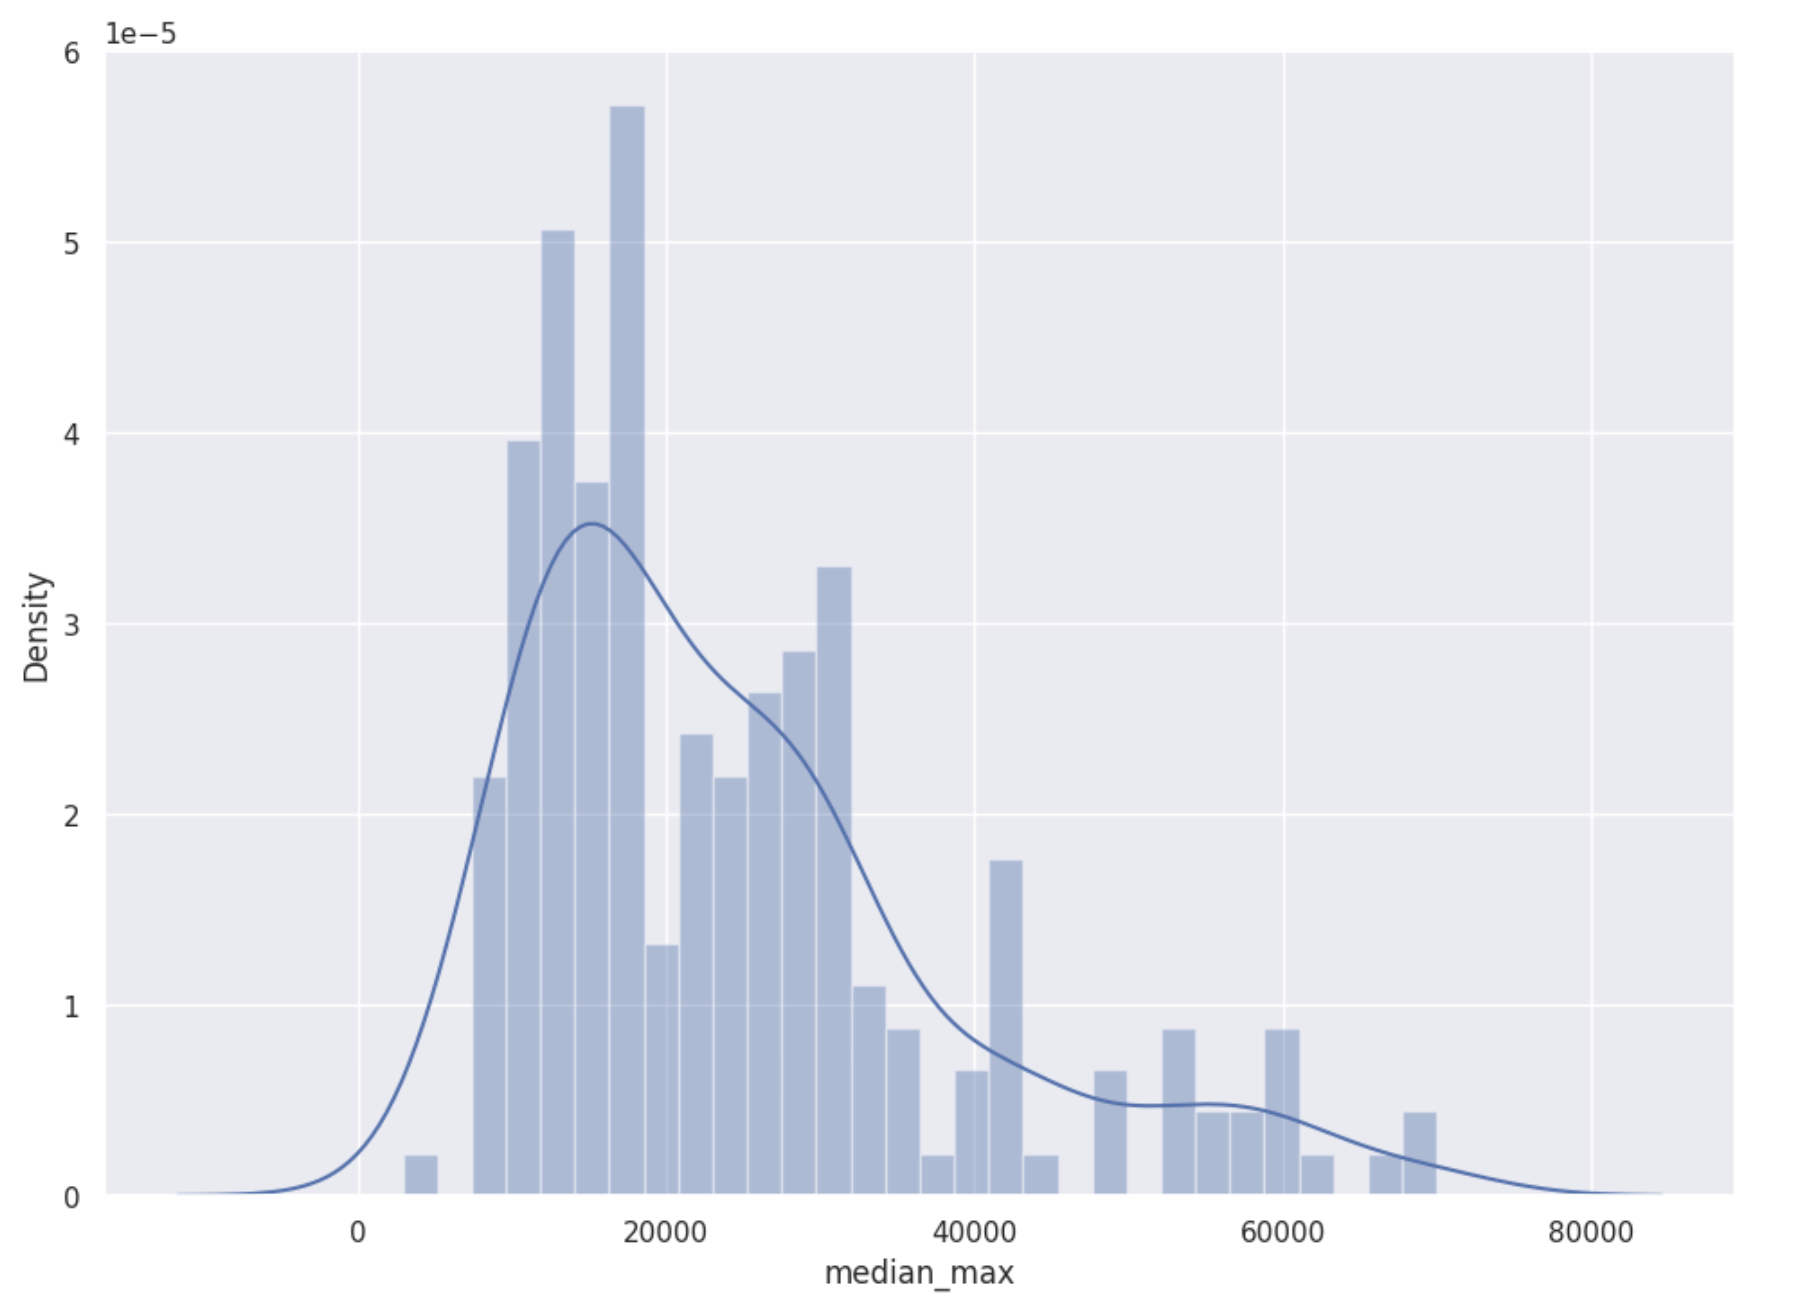
\includegraphics[width=0.6\textwidth, center]{verteilung_max.png}
    \caption[Verteilung von dem Preis Features \emph{median\_max}]{Verteilung von dem Preis Features \emph{median\_max}}
    \label{img:verteilung_max}
\end{figure}

Anders als bei dem Minimalen Median Preis, kann bei dem Maximalen Median Preis keine Normalverteilung erkannt werden. Hier wirken die Werte recht verstreut.

\begin{figure}[h]
    \centering
    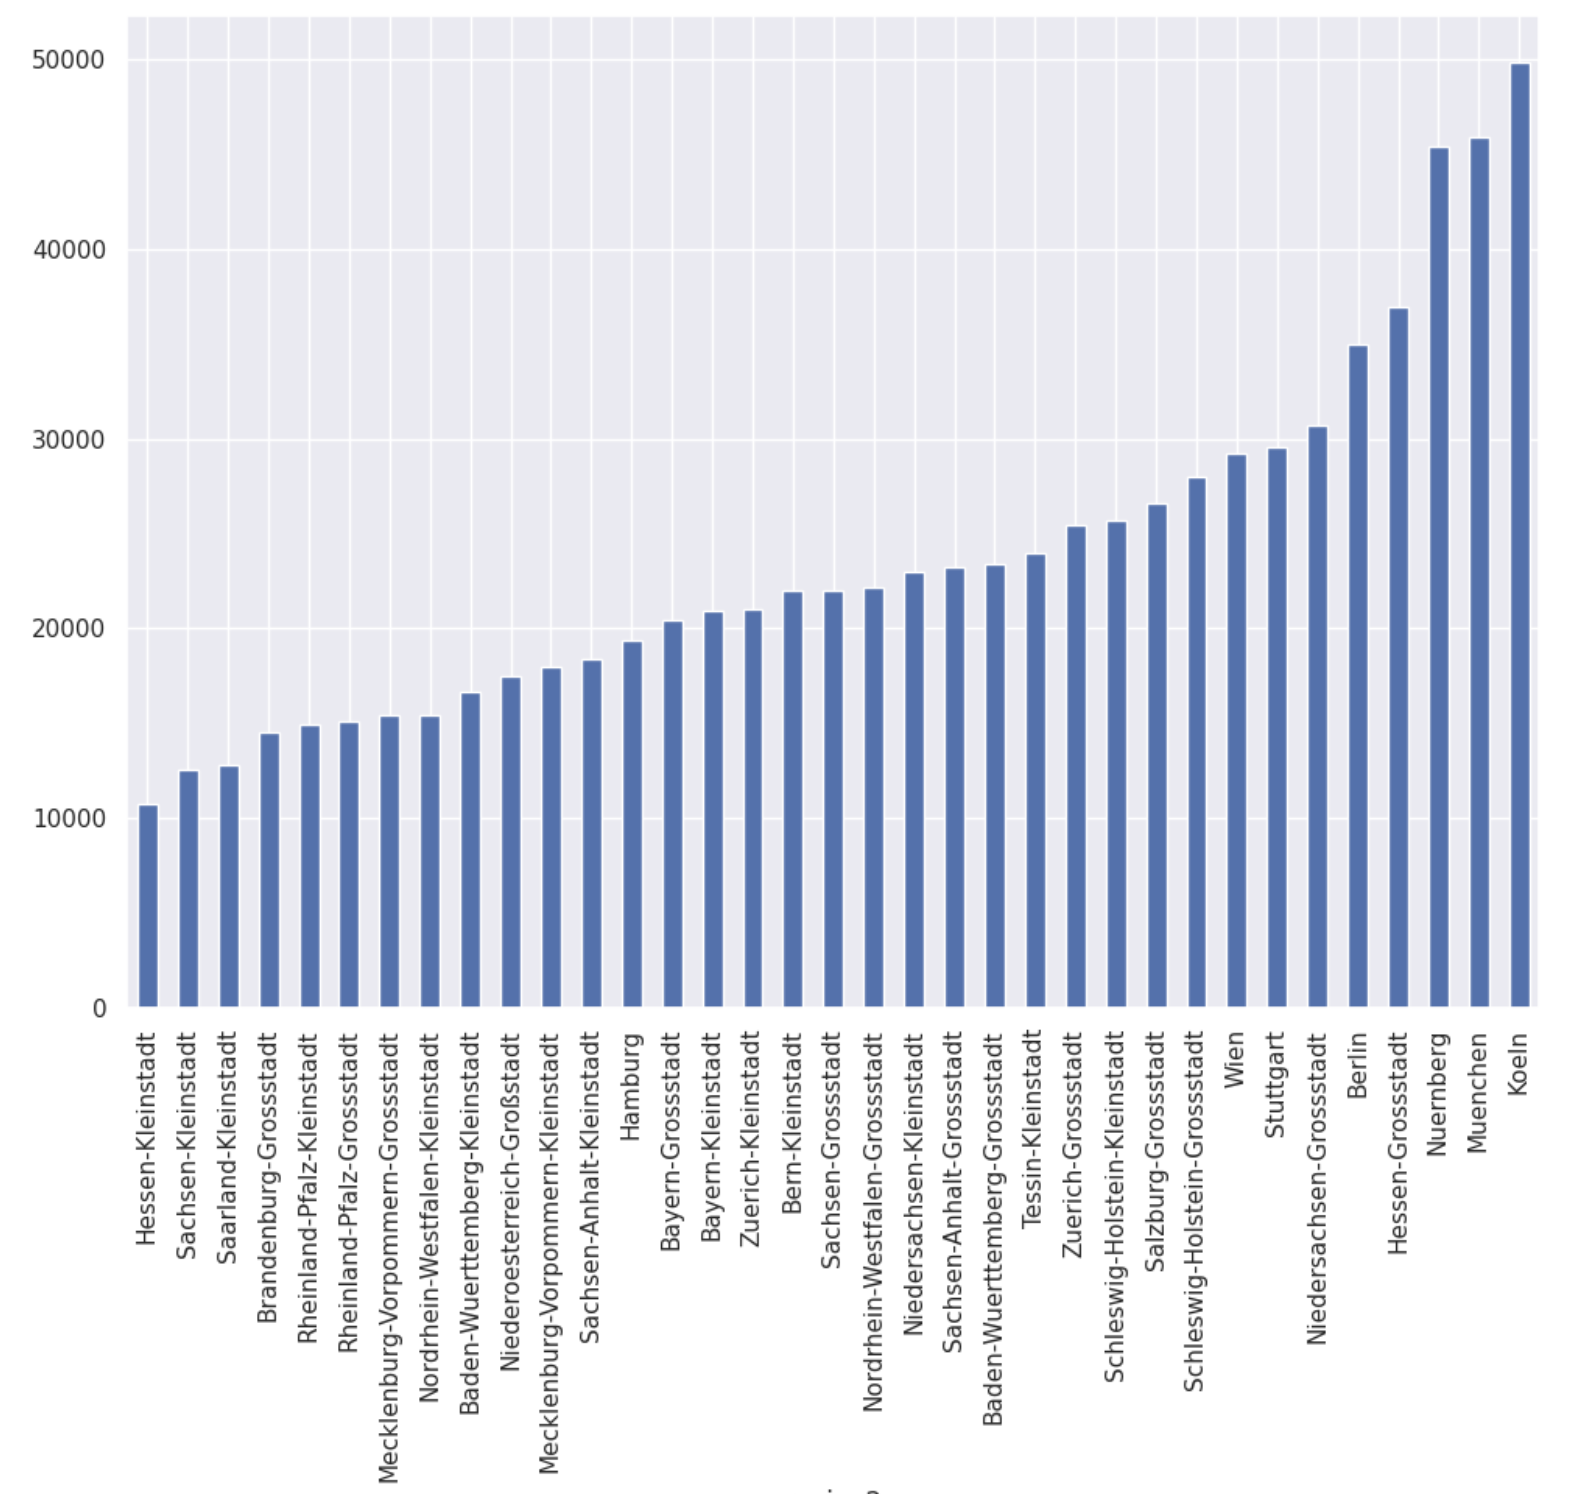
\includegraphics[width=1\textwidth, center]{avg_max_region.png}
    \caption[Durchschnittlicher maximal Preis pro Region]{Durchschnittlicher maximal Preis pro Region}
    \label{img:avg_max_city}
\end{figure}

Abbildung \ref{img:avg_max_city} zeigt, dass es auch deutliche Unterschiede bei den einzelnen Regionen gibt. Eine weitere interessante Erkenntnis ist die, dass es bei dem Maximalen Median Preis eher so ist, dass die Großstädte wie Köln und München eher zu einem höheren Maximalen Preis tendieren.

\subsubsection{Hotelart Feature}
Die Hotelart bildet einen essenziellen Bestandteil, um umfassende Einblicke in die Charakteristiken eines Hotels zu gewinnen. Sie liefert nicht nur Informationen über den Zweck und die Ausrichtung der Unterkunft, sondern ermöglicht auch eine präzise Identifikation der Zielgruppe, die das Hotel anspricht \cite{User.20.01.2024}. Die Zielgruppe eines Hotels ist zudem eine wertvolle Information wenn es darum geht Preise für das Hotel zu gestalten, zumindest ist so die Annahme. Auch in diesem Fall kann wieder nach der Hotelart gruppiert werden und jeweils der Minimale und Maximale durchschnittliche Preis angezeigt werden.

\begin{figure}[h]
    \centering
    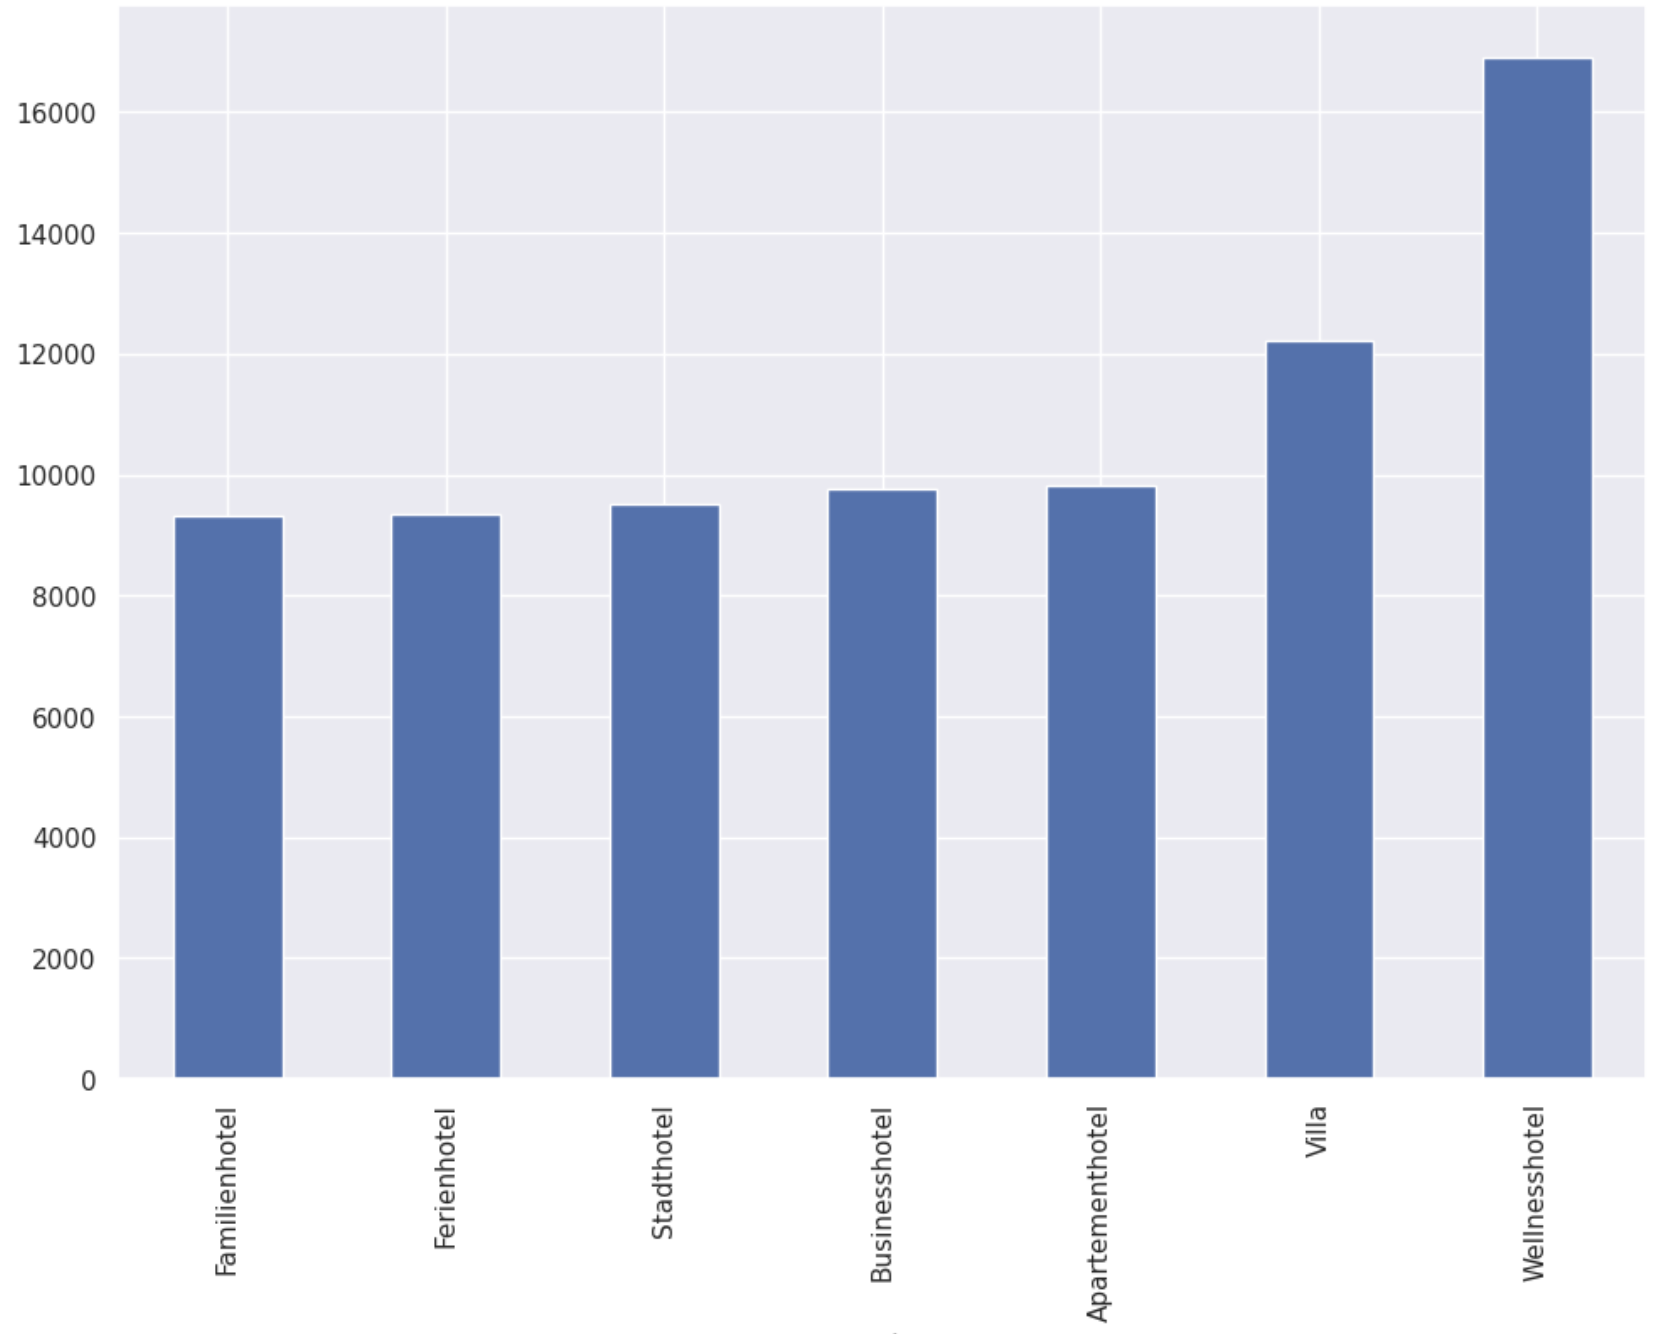
\includegraphics[width=0.6\textwidth, center]{avg_min_art.png}
    \caption[Durchschnittlicher minimal Preis pro Hotelart]{Durchschnittlicher minimal Preis pro Hotelart}
    \label{img:avg_min_art}
\end{figure}

\begin{figure}[h]
    \centering
    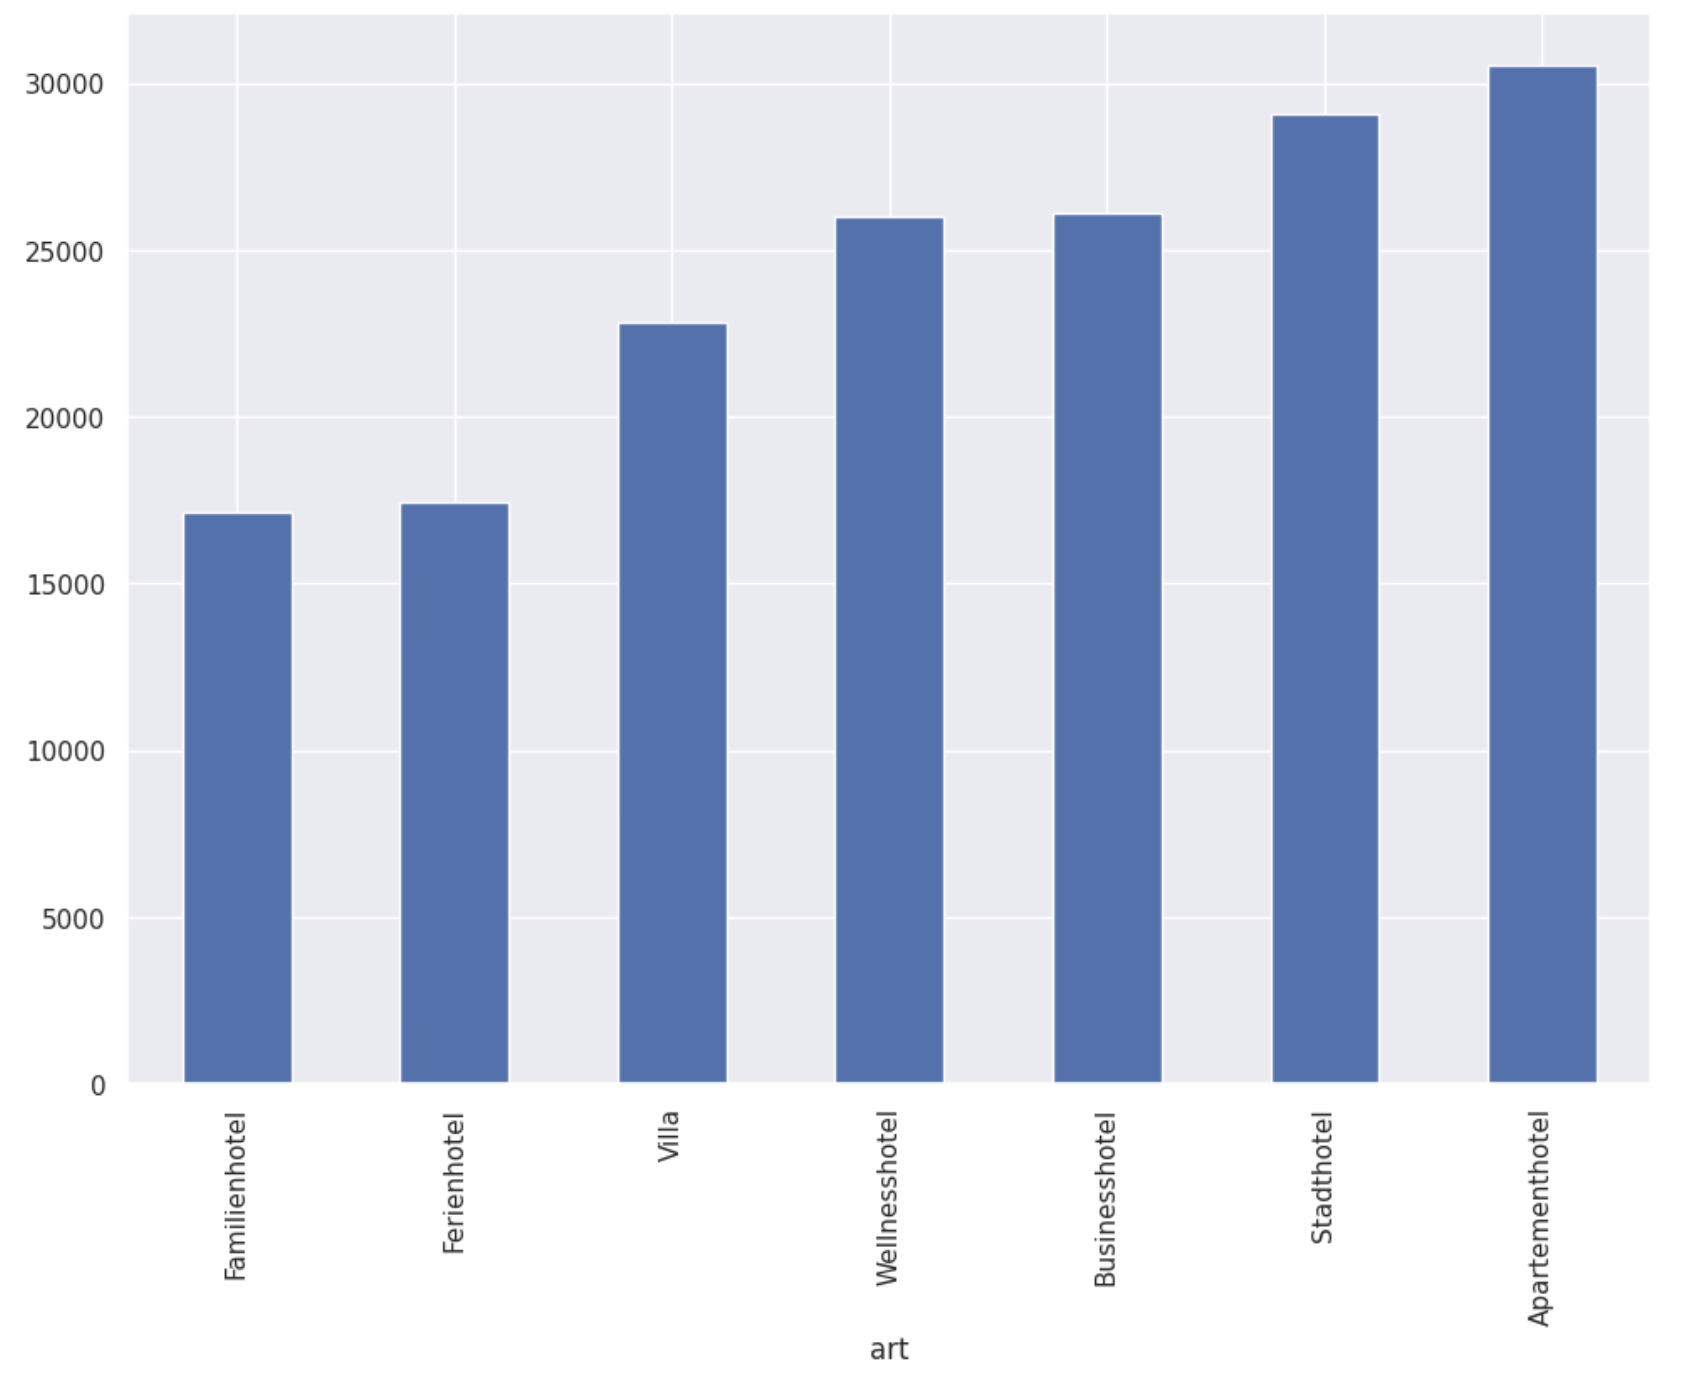
\includegraphics[width=0.6\textwidth, center]{avg_max_art.png}
    \caption[Durchschnittlicher maximal Preis pro Hotelart]{Durchschnittlicher maximal Preis pro Hotelart}
    \label{img:avg_max_art}
\end{figure}

Anhand von den zwei Abbildungen \ref{img:avg_min_art} und \ref{img:avg_max_art} zeigt sich, dass tatsächlich einen unterschied bei den Preisen auf die Hotelart bezogen gibt. Zudem zeigt sich, dass die zwei Hotelarten \emph{Ferienhotel} und \emph{Familienhotel} in beiden Fällen die gleiche Information wiedergibt und somit auch zu \emph{Ferienhotel} zusammengefasst werden kann. Zudem könnten anhand von \emph{median\_min} noch weitere Hotelarten zusammengefasst werden, jedoch wenn beide Informationen zusammen betrachtet werden, so bleibt es lediglich bei \emph{Ferienhotel} und \emph{Familienhotel}.

\subsubsection{Zimmer Features}
Die letzten zwei Features innerhalb des Datensatzes sind die Features \emph{area\_count} und \emph{areatype\_count} welche die Größe des jeweiligen Hotels repräsentieren. Die Frage die sich hier also stellt ist, ob das Preisverhältnis in irgendeiner Art mit der Größe des Hotels zusammenhängen kann. Hierzu soll zunächst auch erstmal die Verteilung der Zimmeranzahl angeschaut werden:

\begin{figure}[h]
    \centering
    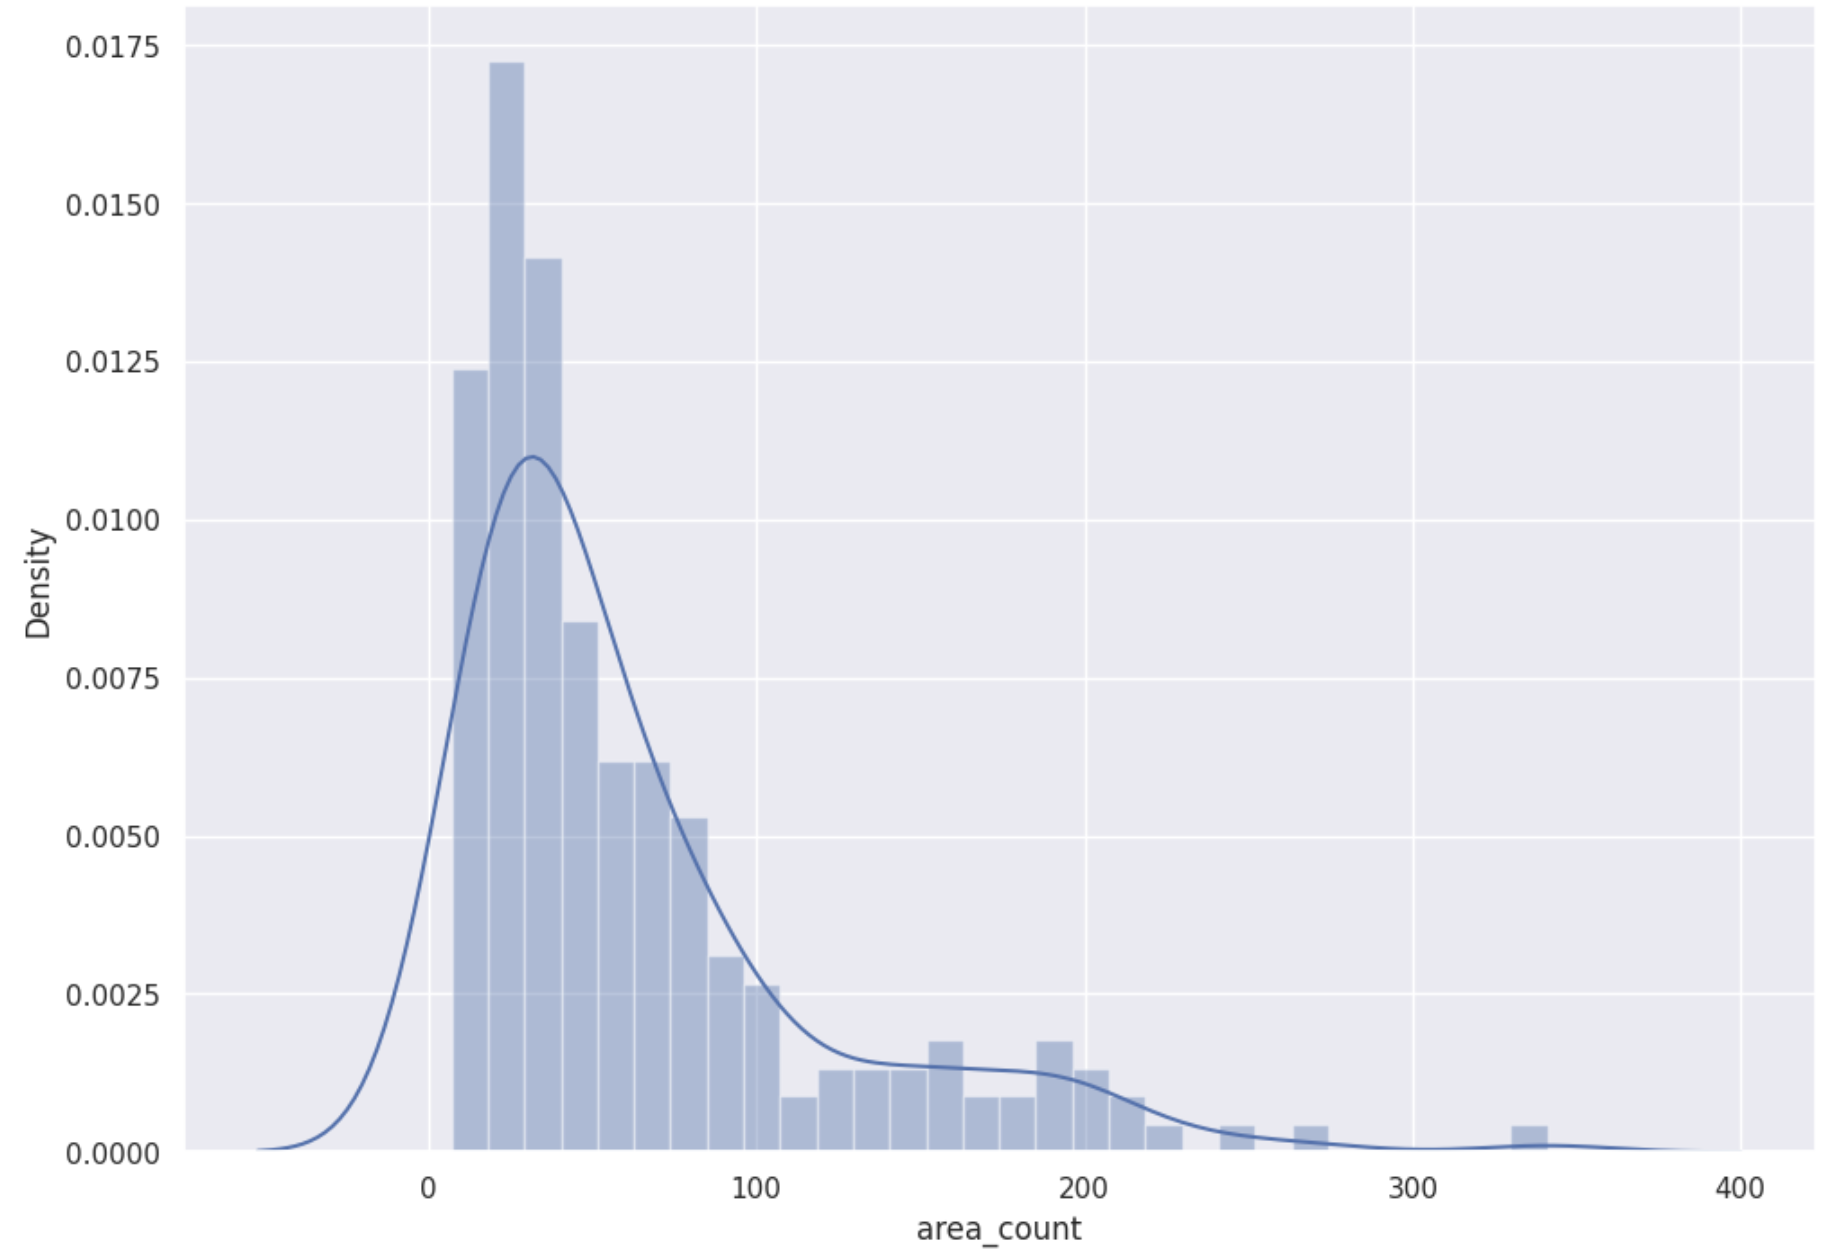
\includegraphics[width=0.6\textwidth, center]{verteilung_area_count.png}
    \caption[Verteilung nach Zimmeranzahl]{Verteilung nach Zimmeranzahl}
    \label{img:verteilung_area_count}
\end{figure}

Die Verteilung zeigt, dass auch recht ausgeprägt ist und nur im Ansatz einer Normalverteilung gleicht. Des Weiteren soll nach der Anzahl der Zimmer gruppiert werden um zu überprüfen wie oft jeder Anzahl vorkommt:

\begin{figure}[h]
    \centering
    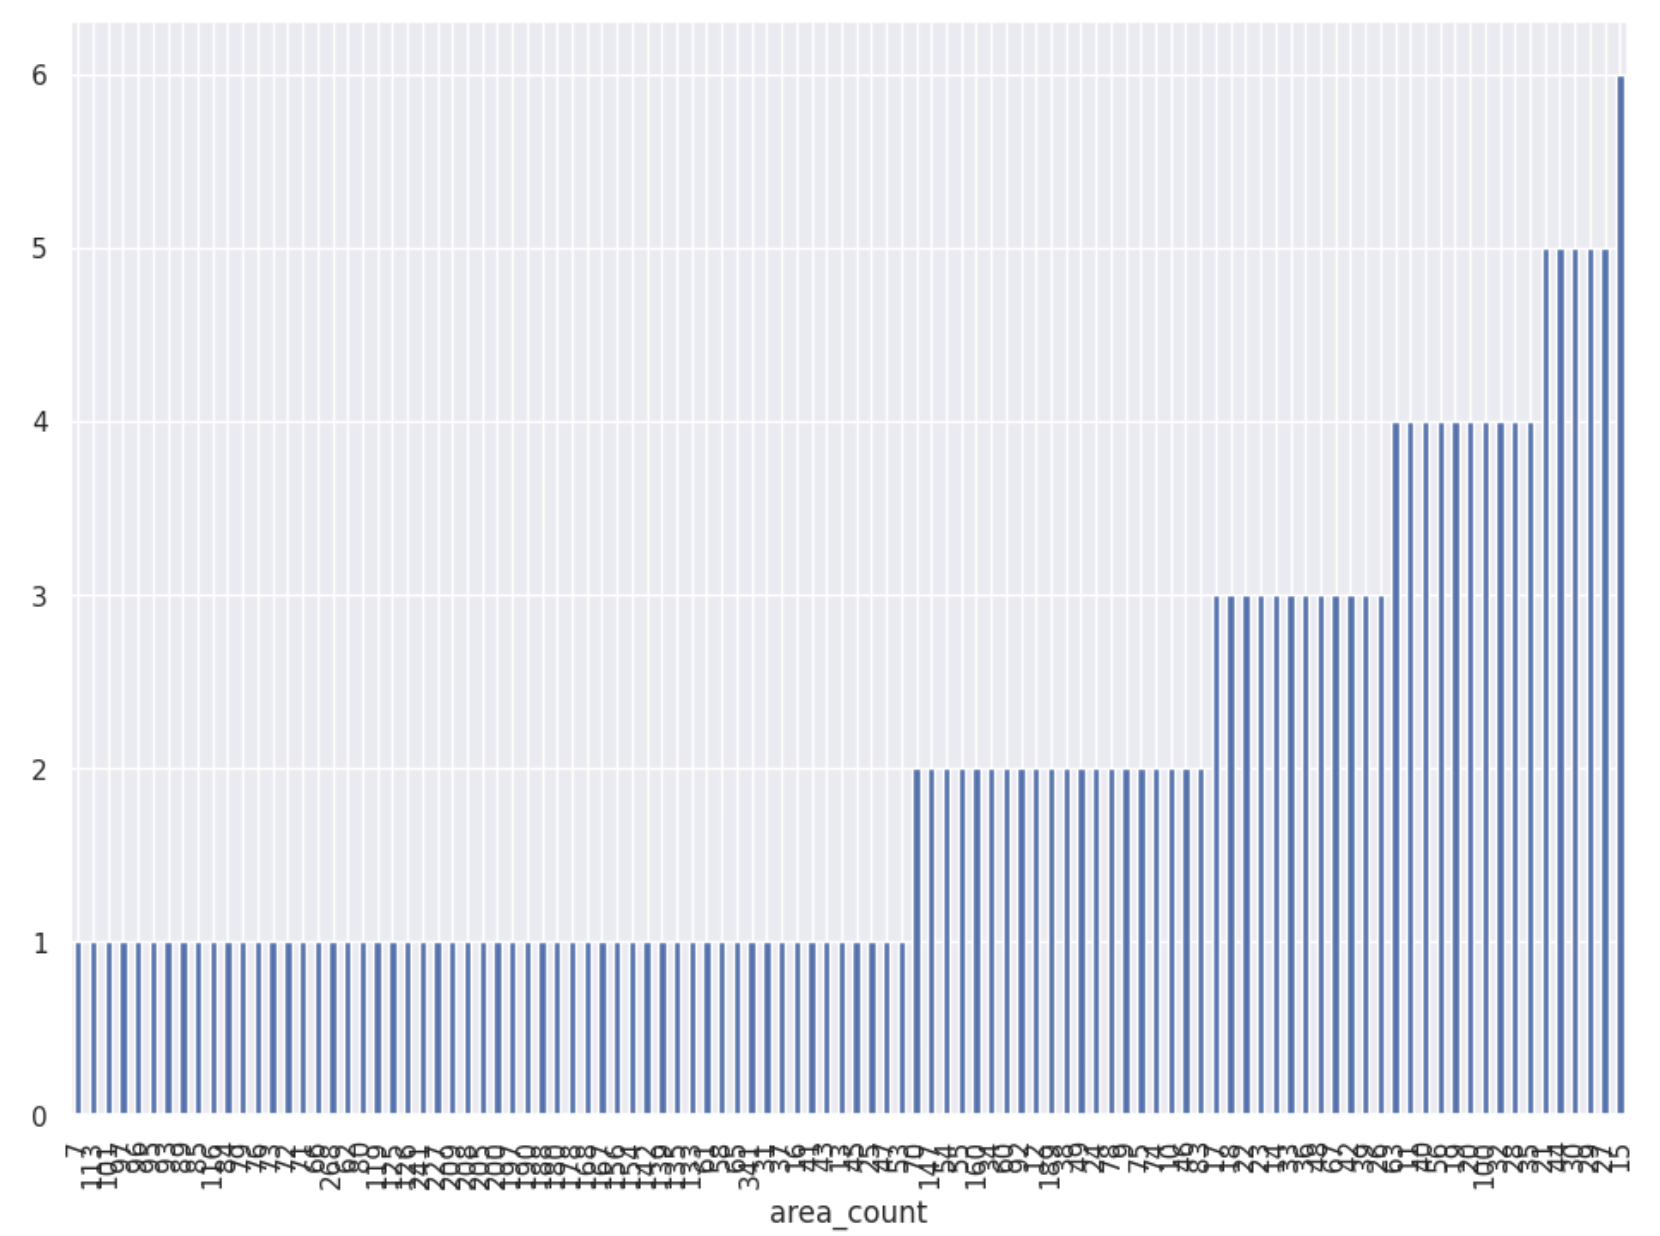
\includegraphics[width=0.6\textwidth, center]{group_area_count.png}
    \caption[Häufigkeit der Zimmeranzahl im Datensatz]{Häufigkeit der Zimmeranzahl im Datensatz}
    \label{img:haufigkeit_area_count}
\end{figure}
Abbildung \ref{img:haufigkeit_area_count} hat gezeigt, dass das Feature \emph{area\_count} zu ausgeprägt ist. Aufgrund dessen, dass das Feature zu ausgeprägt ist und keine Idee vorhanden ist, wie dieses Feature umformuliert werden könnte, wurde beschlossen \emph{area\_count} und \emph{areatype\_count} aus dem Datensatz zu entfernen.
\newline
\newline
Der finale Datensatz welcher für das Modell benutzt werden soll, sieht wie folgt aus:

\begin{figure}[h]
    \centering
    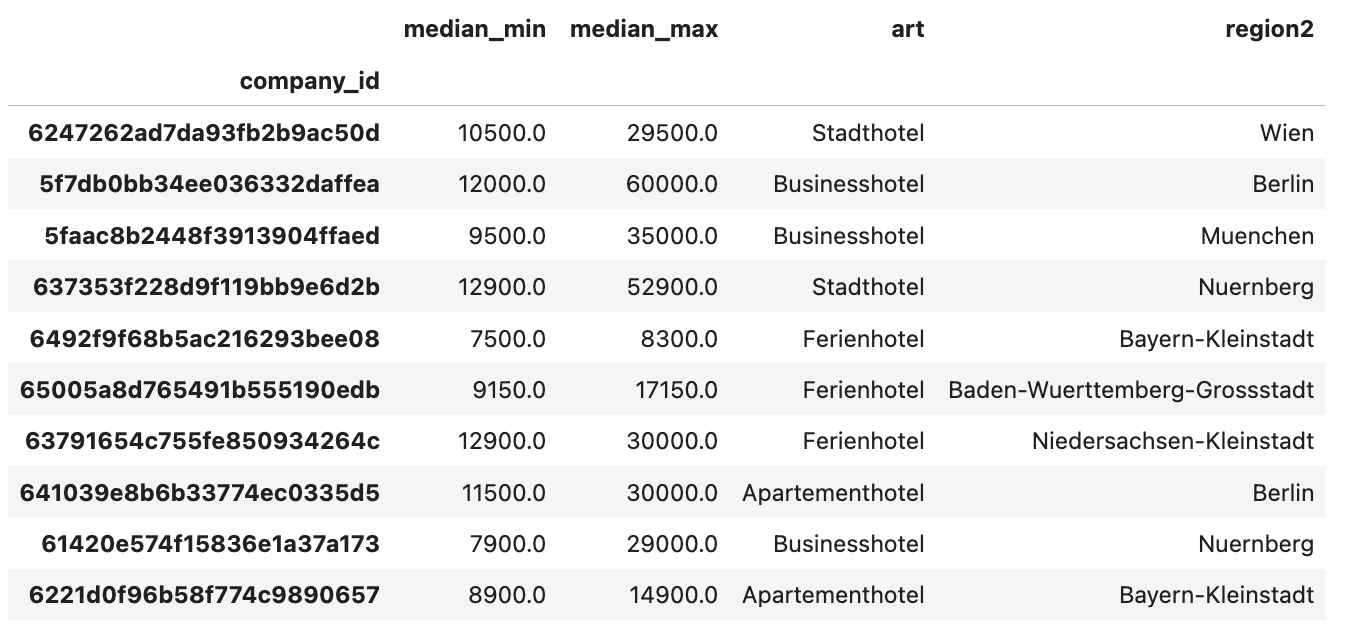
\includegraphics[width=1\textwidth, center]{all_features_4.png}
    \caption[Finaler Datensatz für das Modell]{Finaler Datensatz für das Modell}
    \label{img:all_features_4}
\end{figure}
\subsection{Evaluation der Ähnlichen Hotels}
\label{subsec:Evaluation_1}
Der vorliegende Datensatz ist nun verfügbar, und grundsätzlich kann die Modellierung fortgesetzt werden. Allerdings stellt sich die Frage, ob die identifizierten Hotels tatsächlich ähnlich zum ursprünglichen Hotel sind. Es ist von entscheidender Bedeutung, nachzuweisen, dass die ausgewählten Hotels auf irgendeine Weise miteinander vergleichbar sind. Aus diesem Grund wird im nachfolgenden Abschnitt ein Mechanismus entwickelt, um die Ähnlichkeit der Hotels zu überprüfen und zu gewährleisten.
\newline
\newline
Angesichts des angestrebten Ziels, nämlich der dynamischen Generierung von Preisen, wurde zunächst in Erwägung gezogen, die Preise der einzelnen Hotels zu vergleichen. Zu diesem Zweck wurde initial ein \emph{Dataframe} erstellt, das sämtliche gültigen Hotels sowie ihre Preisinformationen für einen bestimmten Zeitraum umfasst.
\newpage
\begin{figure}[h]
    \centering
    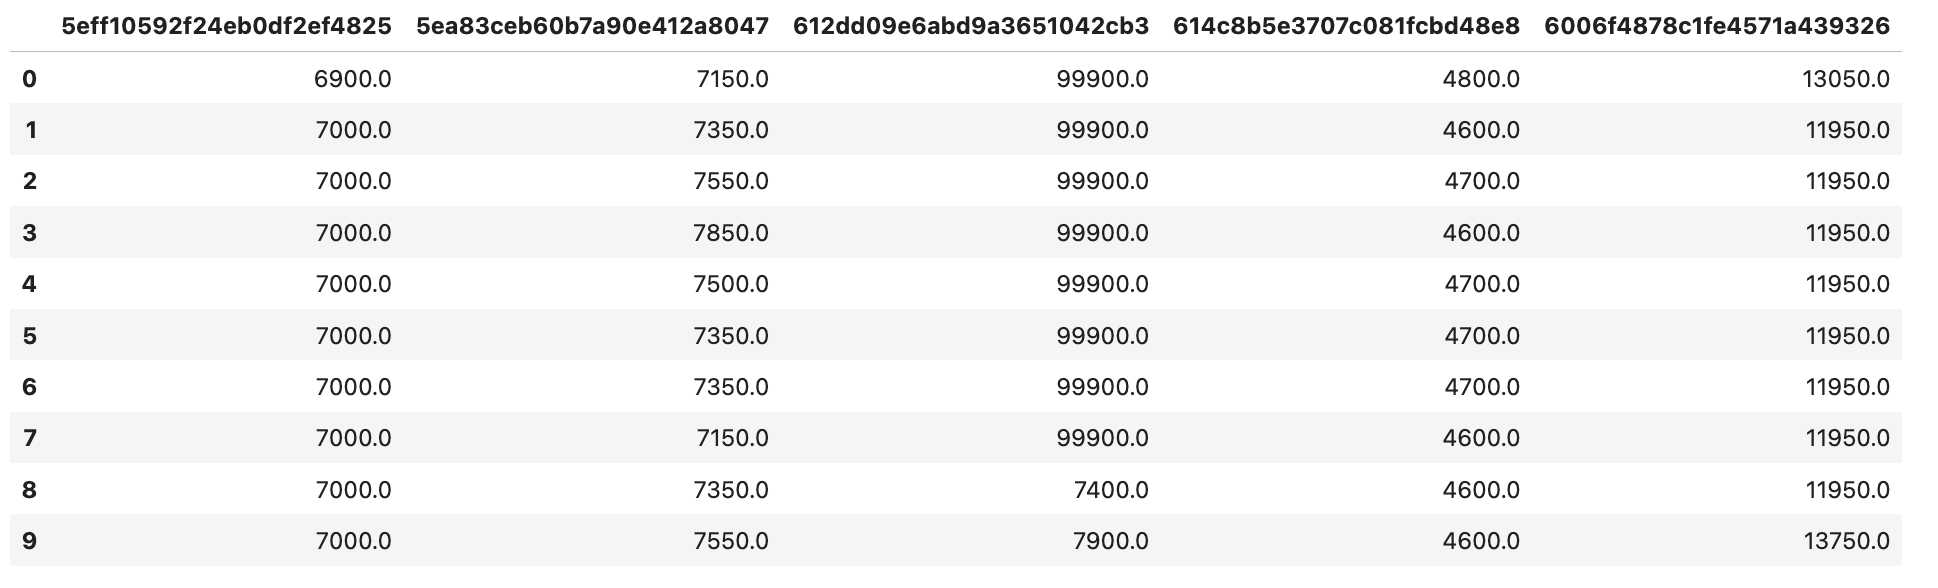
\includegraphics[width=0.9\textwidth, center]{all_prices.png}
    \caption[Preise von allen Hotels für das Jahr 2022]{Preise von allen Hotels für das Jahr 2022}
    \label{img:all_prices}
\end{figure}

Abbildung \ref{img:all_prices} zeigt einen exemplarischen Auszug aus dem DataFrame. Zudem wurde anhand diesem DataFrame noch die dazugehörige Korrelationsmatrix erstellt. Die Korrelationsmatrix ist dafür da um zusammenhänge zwischen den Vektoren zu finden. Dabei beschreibt ein Wert nahe 1 einen hohen positiven Zusammenhang der zwei Vektoren und ein Wert nahe -1 einen hohen negativen Zusammenhang der zwei Vektoren. Ein Korrelationswert gegen 0 beschreibt beschreibt keinerlei Zusammenhang der Vektoren \cite{Team.03.05.2020}. Die Vermutung ist es, dass wenn die Preise von 2 Hotels korrelieren und die Preise sich überschneiden, so werden dass ähnliche Hotels sein. 
\newline
\newline
Diese Vermutung soll dementsprechend mit einigen Hotels getestet werden:
\begin{figure}[h]
    \centering
    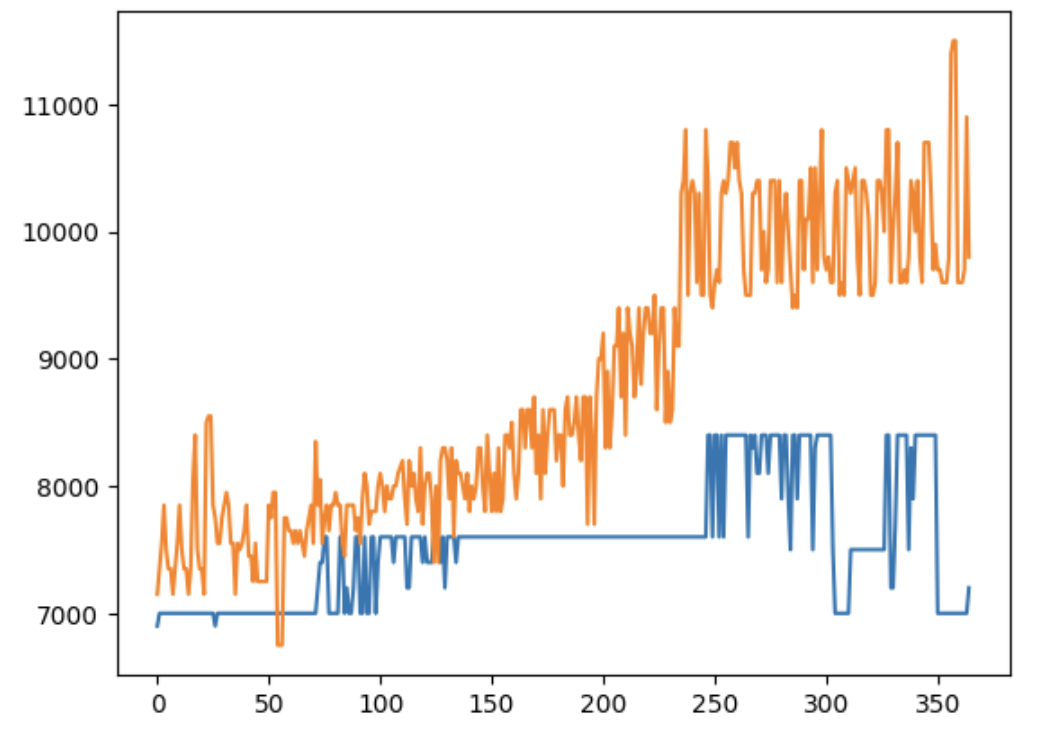
\includegraphics[width=0.9\textwidth, center]{preise_zwei_hotels.png}
    \caption[Visualisierung der Preise zweier Hotels]{Visualisierung der Preise zweier Hotels}
    \label{img:preise_zwei_hotels}
\end{figure}

\begin{figure}[h]
    \centering
    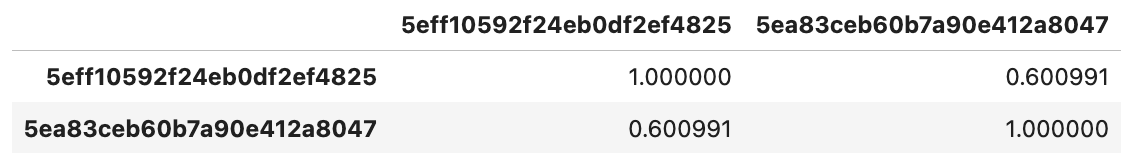
\includegraphics[width=1\textwidth, center]{corr_values_ex.png}
    \caption[Korrelationswerte der zwei Hotels]{Korrelationswerte der zwei Hotels}
    \label{img:corr_values_ex}
\end{figure}

Abbildung \ref{img:preise_zwei_hotels} illustriert den Preisverlauf von zwei Hotels im Jahr 2022, während Abbildung \ref{img:corr_values_ex} die Korrelation zwischen diesen beiden Hotels zeigt. Der festgestellte Korrelationswert von 0,6 erweist sich als bemerkenswert, insbesondere vor dem Hintergrund, dass die Preise in Abbildung \ref{img:preise_zwei_hotels} beträchtlich voneinander abweichen. Infolgedessen wurde die Überlegung angestellt, die Preise zu skalieren und daraufhin miteinander zu vergleichen. Entscheidend für ähnliche Hotels ist lediglich die Tendenz wie sich die Preise verhalten. 
\newline
\newline
Werden die Preise nun Skaliert ändert sich an der Korrelation nichts und die Skalierten Preise sehen nun wie folgt aus:

\begin{figure}[h]
    \centering
    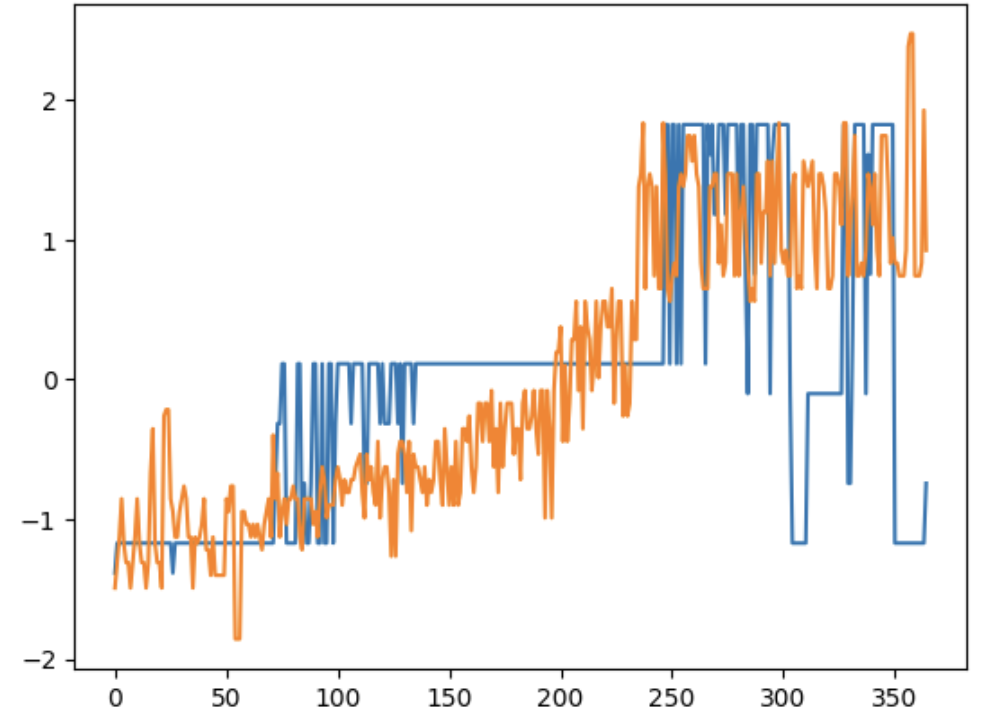
\includegraphics[width=1\textwidth, center]{scaled_preise_zwei_hotels.png}
    \caption[Visualisierung der Skalierten Preise zweier Hotels]{Visualisierung der Skalierten Preise zweier Hotels}
    \label{img:scaled_preise_zwei_hotels}
\end{figure}

Eine zusätzliche Betrachtung ergab die Frage, ob ein ähnliches Muster nicht auch durch die Verwendung des RevPAR erzielt werden könnte. Die Verwendung des RevPAR-Werts erscheint in diesem Kontext sinnvoller als die ausschließliche Berücksichtigung der Zimmerpreise, da das nachfolgende Modell letztendlich darauf abzielt, den RevPAR-Wert vorherzusagen.
\newline
\newline
Im folgenden werden die gleichen zwei Hotels mit dem RevPAR-Wert verglichen:

\begin{figure}[h]
    \centering
    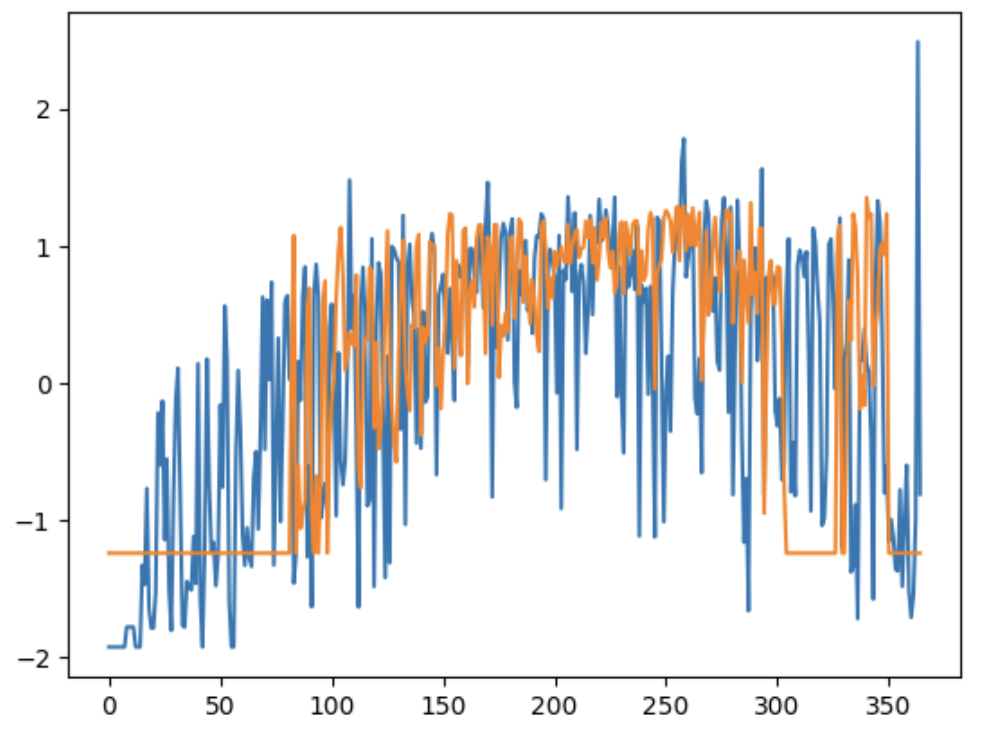
\includegraphics[width=1\textwidth, center]{scaled_revpar_zwei_hotels.png}
    \caption[Visualisierung der Skalierten RevPAR-Werte zweier Hotels]{Visualisierung der Skalierten RevPAR-Werte zweier Hotels}
    \label{img:scaled_revpar_zwei_hotels}
\end{figure}

\begin{figure}[h]
    \centering
    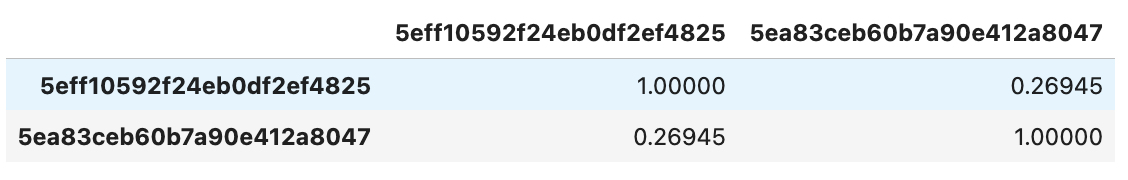
\includegraphics[width=1\textwidth, center]{corr_revpar_values_ex.png}
    \caption[Korrelationswerte der RevPAR-Werte zweier Hotels]{Korrelationswerte der RevPAR-Werte zweier Hotels}
    \label{img:corr_revpar_values_ex}
\end{figure}

Abbildung \ref{img:corr_revpar_values_ex} offenbarte einen abweichenden Korrelationswert im Vergleich zu demjenigen, der bei der Betrachtung der Preisentwicklung ermittelt wurde. Daraufhin wurde die Entscheidung getroffen, dass der Korrelationswert der RevPAR-Werte als aussagekräftiger betrachtet wird als derjenige der reinen Preisentwicklung. Infolgedessen wurde festgelegt, dass dieser Wert als Evaluation für die Ähnlichkeit zwischen den Hotels herangezogen wird.
\newline
\newline
Dieser Korrelationswert der RevPAR-Werte kann lediglich zur Evaluation der Modelle verwendet werden, da dieser Korrelationswert für ein Hotel nicht vorhanden ist. 
\chapter{Unbewachtes Lernen}
\label{subsec:un_lear}
Mit dem konstruierten Datensatz und der zusätzlichen Metrik zur Bestimmung ähnlicher Hotels erfolgt nun die Modellierung. Aufgrund der Unbekanntheit im Vorfeld, welche Hotels miteinander vergleichbar sind, wird ein Modell für unbewachtes Lernen implementiert. Unbewachtes Lernen bezeichnet eine Methode des maschinellen Lernens, bei der der Algorithmus eigenständig und ohne Überwachung Muster sowie Zusammenhänge in den Daten explorativ erkennt \cite{datasolutGmbH.05.02.2024}. Die Grundidee besteht darin, jedes Hotel in einer vergleichbaren Form dem Modell zuzuführen. Dieses Modell erkennt eigenständig Muster und Ähnlichkeiten auf Basis der gegebenen Informationen.
\newline
\newline
Die Evaluation der unterschiedlichen Ansätze und Modelle erfolgt anhand der Benchmark-Hotels, welche in der Sektion zu den Benchmark-Hotels selektiert wurden. Ein Ansatz oder Modell wird als erfolgreich betrachtet, wenn es für die Benchmark-Hotels ein oder mehrere ähnliche Hotels identifiziert, die Korrelationswert von mindestens 0,8 haben.

\input{kapitel/Similar_Hotels/sections/subsections/BasisModel.tex}
\input{kapitel/Similar_Hotels/sections/subsections/dbscan.tex}
\input{kapitel/Similar_Hotels/sections/subsections/doc2vec.tex}
\input{kapitel/Similar_Hotels/sections/subsections/un_fazit.tex}
\subsection{Überwachtes Lernen}
\label{subsec:lean}
Beide unbewachte Ansätze erwiesen sich als nicht zufriedenstellend, dennoch haben sie wertvolle Erkenntnisse geliefert. Es wurde festgestellt, dass die erforderlichen Korrelationswerte für eine Evaluierung vorhanden sind, mit Ausnahme von neuen Hotels ohne entsprechende Daten. Nichtsdestotrotz könnten die bestehenden Korrelationswerte trotzdem genutzt werden, um ein Modell zu trainieren. Die Idee besteht darin, die beschreibenden Merkmale eines Hotels in ein trainiertes Modell einzuspeisen, um die Korrelationswerte vorherzusagen, anstatt direkt ähnliche Hotels zu prognostizieren.
\newline
\newline
Konkret sieht der Ansatz wie folgt aus: Jedes Hotel im Datensatz wird mit jedem anderen Hotel kombiniert, wodurch ein Datensatz der Größe \emph{Anzahl der Hotels x Anzahl der Hotels} entsteht. Zu jeder Kombination wird der Korrelationswert in einer separaten Spalte hinzugefügt, die als Zielvariable für die Vorhersage dient. Ein Modell wird mithilfe dieser Daten und der jeweiligen Zielvariable trainiert. Bei der Vorhersage der Korrelationswerte für ein neues Hotel wird dieses mit jedem anderen Hotel kombiniert und in das Modell eingebracht. Das Modell gibt schließlich die vorhergesagten Korrelationswerte aus.
\newline
\newline
Um diese theoretische Idee zu konkretisieren, werden im folgenden Abschnitt die einzelnen Schritte veranschaulicht.

\subsubsection{Vorbereitung des Datensatzes}
\label{subsubsec:learn_prepare}
Um die beschriebene Idee in die Tat umzusetzen, bedarf es zunächst einer Modifikation des Datensatzes, welcher in Abbildung \ref{img:all_features_4} dargestellt ist. Jede Zeile soll mit jeder anderen Zeile kombiniert werden. Dies wird durch die nachfolgenden Codezeilen realisiert:

\begin{lstlisting}[language=Python, label=lst:learn_prepare, caption=Erstellen des kombinierten Datensatzes]
# Get Hotel ID as seperate column
model_df = model_df.reset_index()
    
# Repeat the rows 2 times
repeat = 2
    
# Get all row combinations 
combinations = list(product(model_df.index, repeat=repeat))
    
# Create the empty result dataframe
combined_df = pd.DataFrame(columns=[f"{column}_{i+1}" for i in range(repeat) for column in model_df.columns])
    
# Combine all combinations in the result dataframe
for combination in combinations:
    row1 = model_df.iloc[combination[0]].values
    row2 = model_df.iloc[combination[1]].values
    new_row = pd.Series(list(row1) + list(row2), index=combined_df.columns)
    combined_df = combined_df.append(new_row, ignore_index=True)
\end{lstlisting}

Mithilfe der im Listing \ref{lst:learn_prepare} präsentierten Codezeilen wurden sämtliche Zeilen erfolgreich miteinander kombiniert. Anschließend kann der Korrelationswert jeder Kombination als neue Spalte \emph{target} hinzugefügt werden.
\newline
\newline
Der resultierende Datensatz, welcher für das Modell verwendet werden soll, sieht wie folgt aus\footnote{Die Hotel-IDs wurden zur besseren Veranschaulichung entfernt}:

\begin{figure}[h]
    \centering
    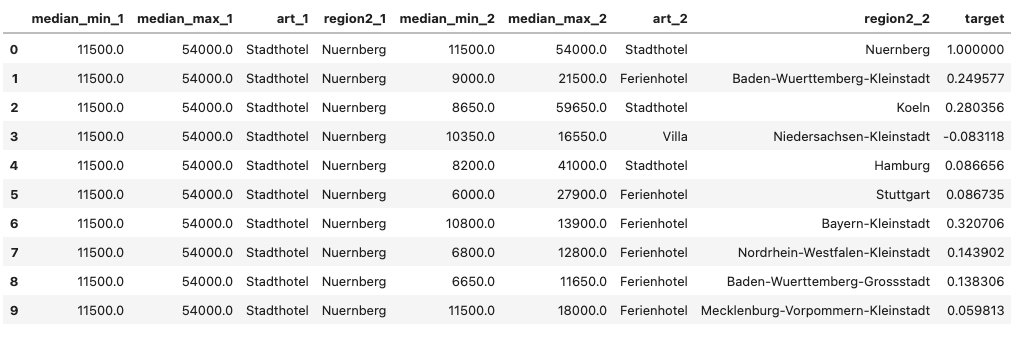
\includegraphics[width=1\textwidth, center]{learn_df1.png}
    \caption[Datensatz bestehend aus den einzelnen Kombinationen]{Datensatz bestehend aus den einzelnen Kombinationen}
    \label{img:learn_df1}
\end{figure}

\subsubsection{Modellbildung}
\label{subsubsec:learn_model}
Für das überwachte Lernen wird CatBoost verwendet, ein hochentwickelter Machine-Learning-Algorithmus, der gezielt auf die Vorhersage von kategorialen Variablen in Datensätzen abzielt und auf dem Gradient Boosting Framework basiert. Eine signifikante Eigenschaft von CatBoost ist seine einzigartige Methode zur Behandlung von kategorialen Merkmalen, bekannt als \emph{Kategorie-Binning}. Diese Methode befähigt den Algorithmus dazu, die internen Strukturen kategorialer Variablen besser zu erfassen und sie effektiv in den Trainingsprozess einzubeziehen, was zu präziseren Vorhersagen führt \cite{Hancock.2020}.
\newline
\newline
Angesichts der Fülle an kategorialen Variablen im vorliegenden Datensatz erweist sich der CatBoost-Algorithmus als besonders geeignet für diese spezifische Aufgabe. Demzufolge kann der Datensatz in seiner aktuellen Form verwendet werden, ohne dass eine umfangreiche Vorverarbeitung erforderlich ist.
\newline
\newline
Im folgenden Abschnitt werden die erforderlichen Codezeilen präsentiert, um das Modell zu trainieren und Vorhersagen für das Benchmark-Hotel zu generieren:

\begin{lstlisting}[language=Python, label=lst:learn_model_train, caption=Erzeugung der Vorhersagen von ähnlichen Hotels mittels CatBoost]
# Get test data
test = combined_df[combined_df["company_id_1"] == str(benchmark_hotel_id)]
# Get train data
train = combined_df.drop(combined_df[(combined_df["company_id_1"] == str(benchmark_hotel_id)) | (combined_df["company_id_2"] == str(benchmark_hotel_id))].index)
# Get X and y from test and train
y_train = train["target"]
X_train = train.drop("target", axis=1)
y_test = test["target"]
X_test = test.drop("target", axis=1)
# Save important informations
hotel_test_df = X_test[["company_id_1", "company_id_2"]]
hotel_test_df["target"] = list(y_test)
# Drop Company ID
X_train = X_train.drop(['company_id_1', "company_id_2"], axis=1)
X_test = X_test.drop(['company_id_1', "company_id_2"], axis=1)
# Define cat features 
cat_features = ["art_1", "region2_1", "art_2","region2_2"]
# Define and train model 
model = cb.CatBoostRegressor()
model.fit(X_train, y_train, cat_features=cat_features)
# Get predictions 
y_pred = model.predict(X_test)
# Add predictions to the information df
hotel_test_df["predictions"] = list(y_pred)
\end{lstlisting}

Mithilfe der Codezeilen im Listing \ref{lst:learn_model_train} wurde ein zusätzliches DataFrame erstellt, das die Hotel-IDs sowie deren Vorhersagen enthält. Dieses DataFrame wird im Folgenden präsentiert:

\begin{figure}[h]
    \centering
    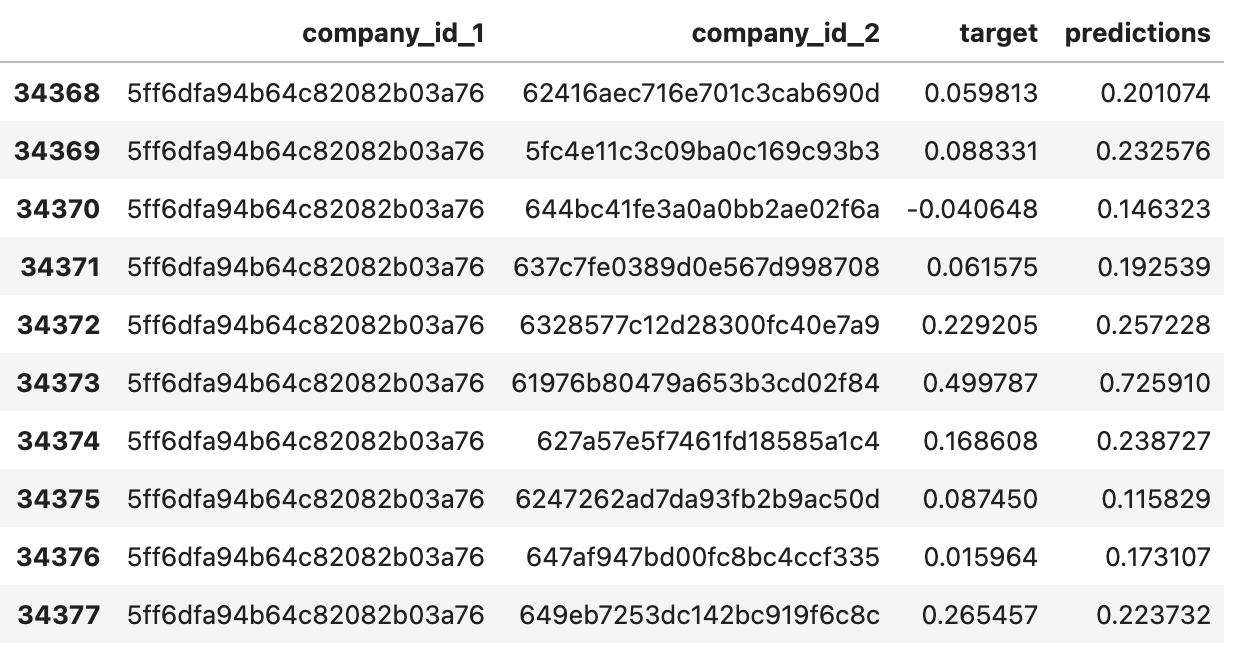
\includegraphics[width=1\textwidth, center]{catboost_similar_results.png}
    \caption[Datensatz der Hotel-IDs und deren Korrelationswert]{Datensatz der Hotel-IDs und deren Korrelationswert}
    \label{img:catboost_similar_results}
\end{figure}

Es besteht nun die Möglichkeit, verschiedene Operationen auf dem DataFrame auszuführen. Zum Beispiel kann auf dem DataFrame gemäß der Bedingung in Abschnitt \emph{\nameref{subsec:un_lear}} gefiltert werden, die besagt, dass Hotelkorrelationen mit mindestens einem Korrelationswert von 0,8 gefunden werden sollen.

\subsubsection{Evaluation}
\label{subsubsec:learn_eval}
Im Gegensatz zu früheren Modellen wurde bei diesem Modell auf eine umfassende Evaluation verzichtet, da der prognostizierte Korrelationswert ausreichend ist, um ähnliche Hotels zu identifizieren. Es wurde lediglich versucht, den R2-Score mithilfe von Hyperparameteranalysen mittels Random Search 
\cite{AdapRandomSearch4.05.2009} und Grid Search \cite{Liashchynskyi.12.12.2019} zu verbessern.



\section{Finden von ähnlichen Hotels Fazit}
\label{subsec:similar_fazit}
In dieser Sektion wurden verschiedene Ansätze zum Finden von ähnlichen Hotels erforscht, beginnend mit dem Einsatz von unbewachtem Lernen unter Verwendung der Algorithmen DBScan und Doc2Vec. Die Ergebnisse dieser Ansätze waren gemischt, wobei beide Algorithmen gewisse Schwächen aufwiesen, darunter die Tendenz, Hotels als ähnlich zu klassifizieren, die in Wirklichkeit nicht zueinander passten.
\newline
\newline
Im Anschluss wurde der Fokus auf überwachtes Lernen verlagert, wobei der CatBoost-Algorithmus eingesetzt wurde. Dieser Ansatz erwies sich als vielversprechend, da er in der Lage war, eine Vorhersage darüber zu treffen, wie ähnlich Hotels zueinander sind. Die Entscheidung, den CatBoost-Ansatz zu verfolgen, wurde getroffen, da bei diesem Ansatz auch ein Korrelationswert vorhanden ist, an dem sich orientiert werden kann.
\chapter{Fazit}
\label{chap:fazit}

Die vorgestellte Arbeit demonstriert die Möglichkeit der Generierung dynamischer Hotelpreise ohne spezifische Vergangenheitsdaten. Dabei wurden verschiedene Methoden erläutert und ein bestimmter Ansatz detailliert umgesetzt. Im gewählten Vorgehen wurden zunächst ähnliche Hotels identifiziert und anhand ihrer Daten ein CatBoost-Modell trainiert, um dynamische Preise für ein Hotel ohne historische Daten zu erzeugen.
\newline
\newline
Des Weiteren wurde ein Vergleich zwischen dem präsentierten Modell und dem aktuellen Live-Modell durchgeführt. Dieser Vergleich zeigt, dass das vorgestellte Modell trotz des Fehlens spezifischer Hotelinformationen mit dem Live-Modell mithalten konnte.
\chapter{Ausblick}
\label{chap:ausblick}
Im Folgenden wird ein kurzer Ausblick auf die weitere Entwicklung der Dynamischen Preisgestaltung von Hotels ohne spezifische Vergangenheitsdaten gegeben. Das ausführlich ausgearbeitete Konzept hat sich als äußerst effektiv erwiesen, um Preise für ein Hotel ohne spezifische Vergangenheitsdaten zu generieren.
\newline
\newline
Es ist jedoch wichtig anzumerken, dass das vorgestellte Konzept nicht in der Lage ist, den Fall zu bewältigen, wenn keine ähnlichen Hotels gefunden werden können. In solchen Fällen bedarf es eines alternativen Konzepts, um Preise zu generieren.
\newline
\newline
Des Weiteren haben weitere Analysen ergeben, dass das Konzept nicht nur für Hotels ohne spezifische Vergangenheitsdaten verwendet werden kann, sondern auch für Hotels mit Vergangenheitsdaten, um noch präzisere Preisgestaltungen zu ermöglichen.

\label{lastpage}

% Neue Seite
\cleardoublepage

% Backmatter mit normalem Zeilenabstand setzen
\singlespacing

% Römische Ziffern für die "Back-Matter", fortlaufend mit "Front-Matter"
\pagenumbering{roman}
%\setcounter{page}{\value{frontmatterpage}}
\setcounter{page}{0}
% Abkürzungsverzeichnis
%\addchap{\hsmaabbreviations}
%\begin{acronym}[IEEE]
	\acro{cd}[CD]{Continuous Delivery}
	\acro{ci}[CI]{Continuous Integration}
	\acro{gui}[GUI]{Graphical User Interface}
	\acro{moc}[moc]{meta object compiler}
	\acro{spa}[SPA]{Single Page Application}
\end{acronym}


% Tabellenverzeichnis erzeugen
\cleardoublepage
\phantomsection
\addcontentsline{toc}{chapter}{\hsmalistoftables}
\listoftables

% Abbildungsverzeichnis erzeugen
\cleardoublepage
\phantomsection
\addcontentsline{toc}{chapter}{\hsmalistoffigures}
\listoffigures

% Listingverzeichnis erzeugen
\cleardoublepage
\phantomsection
\addcontentsline{toc}{chapter}{\hsmalistings}
\lstlistoflistings

% Literaturverzeichnis erzeugen
\begin{flushleft}
\printbibliography[heading=bibintoc, title={Literatur}]
\end{flushleft}

% Index ausgeben. Wenn Sie keinen Index haben, entfernen Sie einfach
% diesen Teil.
%\cleardoublepage
%\phantomsection
%\addcontentsline{toc}{chapter}{\hsmaindex}
%\printindex

% Anhang. Wenn Sie keinen Anhang haben, entfernen Sie einfach
% diesen Teil.
%\appendix
%\chapter{Anhang}
\label{appendix:anhanga}
Test 

\end{document}
